\documentclass[11pt]{article}

% Compile with XeLaTeX (required for CJK body text)
% xelatex -synctex=1 mist_main.tex && bibtex mist_main && xelatex -synctex=1 mist_main.tex && xelatex -synctex=1 mist_main.tex

\usepackage[review]{acl}
\usepackage[UTF8,fontset=none]{ctex}   % Chinese support; requires XeLaTeX
% Synthesize missing bold/italic CJK shapes to suppress "font shape not available" warnings
\setCJKmainfont{Songti SC}[AutoFakeBold=2, AutoFakeSlant=0.2]
\setCJKsansfont{Heiti SC}[AutoFakeBold=2]
\renewcommand{\abstractname}{Abstract}
\renewcommand{\figurename}{Figure}
\renewcommand{\tablename}{Table}
\usepackage{latexsym}
% [T1]{fontenc} and [utf8]{inputenc} are redundant with XeLaTeX+ctex and cause warnings
\usepackage{microtype}
\usepackage{amsmath, amssymb, amsthm}
\usepackage{bm}
\usepackage{graphicx}
\usepackage{booktabs}
\usepackage{multirow}
\usepackage{makecell}
\usepackage{siunitx}
\sisetup{detect-weight=true}
\usepackage{float}
\usepackage{placeins}
\usepackage[dvipsnames, svgnames, x11names]{xcolor}
\usepackage{colortbl}
\usepackage{algorithm}
\usepackage{algpseudocode}
\usepackage{enumitem}
\usepackage{hyperref}
\usepackage{bookmark}   % suppresses rerunfilecheck warning about .out changes
\usepackage{tikz}
\usetikzlibrary{arrows,arrows.meta,positioning,calc}
\usepackage{pgfplots}
\pgfplotsset{compat=1.18}
\usepackage{cancel}
\definecolor{linkblue}{HTML}{000099}
\hypersetup{colorlinks=true,linkcolor=linkblue,urlcolor=linkblue,citecolor=linkblue}
\definecolor{mist}{RGB}{230,220,245}    % highlight: MIST row (w/ RL block)
\definecolor{rlbg}{RGB}{245,243,250}    % highlight: other w/ RL block rows
% Figure~6 strategy-quality bars: light blue / neutral / light purple (match NavyBlue + MediumPurple palette)
\definecolor{qualityQwen}{HTML}{C5DCF5}
\definecolor{qualityTie}{HTML}{EDE9F5}
\definecolor{qualityGPT}{HTML}{D8C8EC}

% ---------- macros ----------
\usepackage{pifont}
\newcommand{\cmark}{\ding{51}}  % ✓
\newcommand{\xmark}{\ding{55}}  % ✗
\newcommand{\gist}{\textbf{GIST}}
\newcommand{\mist}{\textbf{GIST}}  % legacy alias; all new code should use \gist
% \textnormal resets font weight before \textsc, avoiding missing bx/sc (bold small-caps) shape
\newcommand{\sg}{\textnormal{\textsc{SG}}}
\newcommand{\as}{\textnormal{\textsc{AS}}}
\newcommand{\proxy}{\widehat{u}}        % grounded proxy shorthand
\newcommand{\cdash}{---}                % pending-result placeholder in tables
% Method icon macros: left symbol = shot (○=0-shot, ●=few-shot)
%                     right symbol = strategy (○=direct, ●=strategy-then-answer)
\newcommand{\zs}{\ensuremath{\circ\!\circ}}     % 0S:   K=0, direct
\newcommand{\ho}{\ensuremath{\bullet\!\circ}}   % H-0S: K=0, strategy
\newcommand{\fs}{\ensuremath{\circ\!\bullet}}   % FS:   K>0, direct
\newcommand{\hf}{\ensuremath{\bullet\!\bullet}} % H-FS/GIST: K>0, strategy
% Inline Δ% helpers for OOD column
\newcommand{\dg}[1]{{\scriptsize\textcolor{gray}{$#1$\%}}}       % gray Δ (H-0S)
\newcommand{\dr}[1]{{\scriptsize\textcolor{BrickRed}{$+#1$\%}}}  % red Δ (H-FS/MIST)

% ============================================================
% TODO: Replace title with the chosen option (see suggestions below)
%
%  Option A – MIST (revised expansion)
%    "MIST: Training LLMs to Meta-Inductively Solve Problems via
%     Cross-Task Reinforcement Learning"
%    (MIST  Meta-Inductive Skill Training  /  Strategy Transfer)
%
%  Option B – MIND
%    "MIND: Decoupling Meta-Induction from Execution for
%     Generalizable Few-Shot Reasoning"
%    (MIND = Meta-INductive Decoupling)
%
%  Option C – LIRA
%    "LIRA: Learning to Induce Reusable Abstractions via
%     Cross-Task Reinforcement Learning"
%    (LIRA = Learn-to-Induce via RL Alignment)
%
%  Option D – COIN
%    "COIN: Cultivating Cognitive Induction Habits in LLMs via
%     Cross-Task RL"
%    (COIN = COgnitive INduction training)
%
%  Option E – HABIT
%    "HABIT: Hierarchical Alignment-Based Inductive Training for
%     Few-Shot Generalization"
%    (HABIT = Habit-Aligned Bi-level Inductive Training)
% 
%  MIST: Cultivating Meta-Inductive Habits in Large Language Models via
%  Cross-Task Reinforcement Learning
% ============================================================
\title{GIST: Generalization through Inductive Strategy Transfer via Query-Blind Decoupled Reinforcement Learning}

\author{Anonymous Author \\
  Anonymous Institution \\
  \texttt{anonymous@domain}}

\begin{document}
\maketitle

% ============================================================
\begin{abstract}
{\fontsize{10pt}{12pt}\selectfont
When humans encounter unfamiliar problems, they naturally abstract a reusable strategy from
examples before applying it; in-context learning (ICL), despite its powerful few-shot
adaptation, folds this induction step implicitly into execution, leaving LLMs'
meta-inductive capability latent and untapped.
We propose \mist{} (Meta-Inductive Strategy Training) to elicit this intrinsic capability,
operationalizing ``induce first, execute second'' via cross-task reinforcement learning
without strategy annotations.
\mist{} decouples a query-blind Strategy Generator (\sg{}) from a frozen Answer Solver (\as{})
via gradient partitioning, trained across 110+ tasks under a multiplicative reward combining
difficulty-aware Execution Improvement (EIR) and Internal Confidence (ICR) measuring
the strategy's effect on \as{}'s decoding distribution.
On BIG-Bench (ID/OOD) and BIG-Bench Hard, \mist{}-4B (Qwen3-4B) achieves $+120\%$ relative
ID and $+84\%$ OOD accuracy gains over few-shot ICL; models further attain $+57\%$ OOD
\emph{absent the strategy step}, confirming that \mist{} reconfigures latent inductive
representations rather than appending an auxiliary capacity.
}
\end{abstract}
% ============================================================
\section{Introduction}
\label{sec:intro}

\begin{figure}[t!]
\centering
\includegraphics[width=\columnwidth]{figure/fig1_new.png}
\caption{%
  \textbf{ICL} (left) folds induction into execution, coupling inductive signals to surface query patterns and degrading OOD generalization.
  \textbf{\gist{}} (right) decouples the two: query-blind \sg{} induces strategy $s$ from demonstrations; frozen \as{} executes $s$ on the query.
}
\label{fig:overview}
\end{figure}

% ── 第一部分：大背景与问题动机 ──
从少量示例中归纳可迁移的策略并将其复用于新问题，是人类认知泛化的核心机制之一。大语言模型（LLM）通过上下文学习（ICL）展现出强大的少样本适应能力~\citep{brown2020gpt3}，其中内在地蕴含着这一元归纳潜力，即从示范中提炼任务级可复用策略的能力。然而，标准 ICL 将规律归纳与答案执行压缩为单次前向传播~\citep{xie2022icl_bayesian,akyurek2023icl_algorithm}，使模型仅能捕捉与查询表面形式紧耦合的浅层对应，而非真正提取抽象可迁移规律，内在的元归纳能力因此长期潜伏而未被充分利用~\citep{li2025mirage,zhou2024selfdiscover}。这一局限导致 LLM 在输入分布偏移下泛化能力显著下滑~\citep{min2022rethinking,wang2024icl_ood}。如何有效提升 LLM 的元归纳能力，使其从示范中真正提取出可跨任务复用的抽象策略，正是本文所要解决的核心问题。

% ── 第二部分：现有方法的局限性 ──
对 LLM 归纳推理的专项评测揭示了一个关键不对称性~\citep{li2025mirage}：LLM 是出色的 neighbor-based reasoner，能有效捕捉示例与查询间的表层对应；却非合格的 rule-based reasoner，语义对应减弱时归纳准确率大幅下滑。这一发现直接指向标准 ICL 的结构性悖论，ICL 本身正是依赖 neighbor-based 机制将归纳与执行压缩为单次前向传播~\citep{xie2022icl_bayesian,akyurek2023icl_algorithm}，绑定于具体输入分布，在 OOD 场景下导致系统性准确率退化~\citep{min2022rethinking,wang2024icl_ood}。思维链与结构化推理~\citep{wei2022cot,zhou2024selfdiscover}引入可见中间步骤，但推理轨迹以具体查询为条件生成，本质上仍是 query-level 答案路径而非跨样本可复用的任务级归纳先验，其局限与 ICL 同根同源。自动化提示优化~\citep{zhou2023ape,yang2024opro,fernando2023promptbreeder,agrawal2025gepa}在形式上分离了归纳与执行，却将优化对象绑定于单任务实例分布，缺乏将归纳机制跨任务固化的训练信号，OOD 泛化收益不稳定。综上，现有方法均未能为 LLM 提供在分布偏移下真正鲁棒的\textbf{查询无关任务级归纳表征}。

OOD 泛化的障碍，不在于缺乏中间推理步骤，而在于缺乏\textbf{查询无关的任务级归纳表征}，即仅从示范中提炼、独立于具体查询、在分布偏移下依然鲁棒的抽象策略（见图~\ref{fig:overview}）。实现这一目标面临两个技术挑战：（1）在无策略标注的条件下，归纳质量无法被直接监督，模型只能从执行结果中反推“什么是可迁移的策略"；（2）在同任务分布上优化时，模型可通过捕捉示范与查询之间的表面对应绕过真正的抽象，即\textbf{捷径折叠}（shortcut collapse）会导致跨分布泛化脆弱。

% ── 第三部分：本文的直觉与核心方法 ──
为此，我们提出 \mist{}（Meta-Inductive Strategy Training），在多种异构任务上通过跨任务强化学习将“先归纳、后执行"可操作化。针对\textbf{挑战一}，\mist{} 采用\textbf{query-blind双层架构}：可训练的策略生成器（\sg{}）仅从 $K$ 条示范归纳半结构化策略 $s$，全程不接触测试查询，从结构上强制学习任务级抽象而非查询级对应。针对\textbf{挑战二}，\mist{} 引入\textbf{梯度分区}：答案求解器（\as{}）全程冻结，梯度无法经由执行层回传至 \sg{}，从架构上斩断 \sg{} 退化为查询条件前缀触发器的捷径通路。在监督信号上，系统采用联合奖励 EIR$\times$ICR：执行改进奖励（EIR）衡量难度感知的准确率增益，内部置信奖励（ICR）衡量策略对 \as{} 解码分布的影响，两者协同驱动 \sg{} 在无策略标注条件下提升元归纳能力。

% ── 第四部分：实验结果的高亮 ──
在 BIG-Bench（ID/OOD）与 BIG-Bench Hard~\citep{srivastava2023bigbench,suzgun2022bbh} 上，\mist{}-4B（Qwen3-4B）相对 few-shot ICL 实现 $+120\%$ ID 与 $+84\%$ OOD 相对准确率提升，OOD 增益与 ID 高度一致，排除了表面记忆假说。更值得关注的是，推理时移除策略步骤后，隐式 ICL 的 OOD 准确率仍提升 $+57\%$，证明 \mist{} 重构了模型的潜在归纳表征而非仅附加行为模块。在多类 OOD 任务上，\mist{}-4B 与参数量数倍于自身的强基线相当，表明元归纳习惯的习得与模型规模相互正交。

% ============================================================
\section{GIST: A Bi-Level Framework}
\label{sec:method}

设 $\mathcal{T}$ 为异构任务空间；对任务 $\tau \sim P(\mathcal{T})$，$\mathcal{D}_\text{spt}^{(\tau)} = \{(x_i, y_i)\}_{i=1}^{K}$ 为 $K$ 个 few-shot 示例，$(x, y^*) \in \mathcal{D}_\text{qry}^{(\tau)}$ 为测试查询-答案对，目标是从 $\mathcal{D}_\text{spt}^{(\tau)}$ 归纳可复用的任务级策略并显式施用于新查询。标准 ICL 将归纳与执行压缩为单次前向传播，使元归纳能力潜伏于查询特定激活，OOD 泛化因此脆弱~\citep{li2025mirage,min2022rethinking}。\gist{} 将``先归纳、后执行''操作化为梯度分区的双层系统（图~\ref{fig:arch}）：\S\ref{sec:arch} 定义双角色架构；\S\ref{sec:object} 描述推理正向流程；\S\ref{sec:training} 阐明训练信号设计。

\begin{figure*}[t]
\centering
\includegraphics[width=\textwidth]{figure/fig2_new.png}
\caption{%
  Overview of \gist{}.
  \textbf{(a)~Meta-level:} The trainable \sg{} (query-blind) induces a reusable strategy $s_i$ from $K$ demonstrations; gradient partitioning blocks back-propagation from \as{} to \sg{}.
  \textbf{(b)~Object-level:} The frozen \as{} executes $s_i$ on queries, computing EIR (difficulty-adaptive signed accuracy gain) and ICR (token log-probability confidence) as joint reward.
  \textbf{(c)~Training:} SFT cold-starts \sg{}; Phase-2 GRPO optimizes $R_i = R_{\text{EIR},i}{\cdot}(1{+}\beta R_{\text{ICR},i})$ with \as{} frozen throughout.
}
\label{fig:arch}
\end{figure*}

% ============================================================
\subsection{Architecture}
\label{sec:arch}

\gist{} 将单一骨架模型在功能上划分为可训练的策略生成器（\sg{}）与冻结的答案求解器（\as{}），两步生成过程为：
\begin{equation}
\begin{gathered}
  s \;\sim\; \pi_{\sg{}}\!\bigl(\cdot \mid \mathcal{D}_\text{spt}^{(\tau)}\bigr),\\[2pt]
  \hat{y}(s,x) \;\triangleq\; \arg\max_{y}\; P_{\as{}}\!\bigl(y \mid s,\, x\bigr).
\end{gathered}
\label{eq:two_step}
\end{equation}
\sg{} 仅凭支持集归纳策略，全程不接触测试查询（query-blind），强制学习 task-level abstraction 而非 instance-level pattern matching；\as{} 以策略 $s$ 为条件执行求解，两者以显式策略文本 $s$ 为唯一信息通道。两角色共享同一预训练 checkpoint，保证策略的语义空间与 \as{} 的解码先验兼容。

\paragraph{策略格式.}
策略文本 $s$ 由三节强制格式构成：\texttt{[INDUCTIVE\_RULE]}（任务族归纳规律）、\texttt{[TASK\_PROCEDURE]}（3--6 条可执行步骤）、\texttt{[TRANSFER\_SCOPE]}（适用边界），格式违规惩罚纳入奖励设计（\S\ref{sec:training}）。半结构化接口提供稳定 prompt 模板，保证 ICR 对数概率跨样本可比（完整规范见 Appendix~\ref{app:schema}）。

% ============================================================
\subsection{Object-Level}
\label{sec:object}

\paragraph{推理正向流程.}
给定 $\mathcal{D}_\text{spt}^{(\tau)}$，\sg{} 生成策略 $s$；冻结的 \as{} 以 $s$ 为前缀，对每道查询 $x_m$ 执行贪婪解码，输出 $\hat{y}$。\as{} 全程冻结：冻结使执行器映射 $p_\phi(y \mid s, x)$ 在 RL 训练中保持静止，保证奖励函数跨步可比（training stability）；同时使 \S\ref{sec:training} 的 ICR 对数概率跨步具有一致基准（ICR measurability）。由于 $s$ 是离散自然语言接口，梯度无法从 \as{} 回传至 \sg{}（梯度分区），从架构上阻断 \sg{} 退化为依赖激活触发器的捷径策略。

\gist{} 的优化目标
\begin{equation}
  \mathcal{J}_{\text{GIST}} =
    \max_{\pi_{\sg{}}}\;
    \mathbb{E}_{\substack{\tau,\,\mathcal{D}_\text{spt}^{(\tau)}\\(x,\,y^*)}}
    \Bigl[\,
    \mathbb{E}_{s \sim \pi_{\sg{}}}
    \bigl[\mathbb{1}[\hat{y}(s,x) = y^*]\bigr]
    \Bigr]
  \label{eq:j_gist}
\end{equation}
类比于文本空间的双层元学习：外循环以 RL 跨任务优化 $\pi_{\sg{}}$，内循环以单次前向推理生成 $s$，代价 $O(1)$（\textbf{优于 MAML 的 $O(K|\theta|)$ 梯度展开}~\citep{finn2017maml}）。$s$ 以自然语言承载适应信息，与模型参数完全解耦：\textbf{训练时冻结的 \as{} 可在测试时免训练替换为更强求解器}（\S\ref{sec:analysis} 实证验证）。

% ============================================================
\subsection{Meta-Level}
\label{sec:training}\label{sec:reward}

\paragraph{Phase 1：SFT 冷启动.}
在教师生成的格式样本上微调 \sg{}，仅初始化输出格式与基础策略跟随行为，不以任务性能为优化目标；同时以 $\pi_{\sg{}}^{(0)}$ 的推理准确率预填充滚动基线缓冲区 $b_\tau$，使 Phase 2 基线反映``具备格式能力但尚未习得归纳先验''的初始水平（完整配置见 Appendix~\ref{app:training}）。

\paragraph{Phase 2：联合奖励 RL 训练.}
Phase 2 设计两类互补奖励，驱动 \sg{} 在无策略标注条件下习得元归纳能力：\textbf{EIR}（执行改进奖励）以外显准确率增量衡量策略的难度自适应改进；\textbf{ICR}（内部置信奖励）以解码分布收敛程度弥补 EIR 无法区分精准命中与偶然命中的不足。两者以乘性门控组合为联合奖励：
\begin{equation}
  R_i = R_{\text{EIR},i} \cdot \bigl(1 + \beta \cdot R_{\text{ICR},i}\bigr)
  \label{eq:total_reward}
\end{equation}
其中 $\beta = 0.5$（消融见 \S\ref{sec:ablation}）；Phase~2 在 110+ 异构任务上运行 GRPO（$G{=}8$ 并行 rollout，$M{=}4$ 道查询），\as{} 全程冻结。格式不合规的策略获固定惩罚 $R_i = -\lambda_\text{fmt}$，不传入 \as{} 执行。

\paragraph{执行改进奖励（EIR）.}
令 $\delta_i = \bar{A}_i^{(\tau)} - b_\tau$ 为策略 $s_i$ 在 $M$ 道查询上的准确率相对滚动基线 $b_\tau$ 的偏移（奖励以 rollout 前 $b_\tau$ 计算，rollout 后以 EMA 更新，避免 within-group leakage）。难度归一化原始增益 $g_{\text{raw}}$ 定义为：
\begin{equation}
\begin{aligned}
  \bar{A}_i^{(\tau)} &= \frac{1}{M}\sum_{m=1}^{M}
    \mathbb{1}\bigl[\as{}(s_i,\,x_m)=y_m^*\bigr],\\
  \delta_i &= \bar{A}_i^{(\tau)} - b_\tau,\\
  g_{\text{raw}} &= \frac{|\delta_i|}{\max\!\bigl(
    b_\tau^{\alpha}(1{-}b_\tau)^{1-\alpha},\;\varepsilon\bigr)}
\end{aligned}
\label{eq:eir_raw}
\end{equation}
其中 $\alpha = \alpha^+$（$\delta_i \geq 0$）或 $\alpha^-$（$\delta_i < 0$），满足 $\alpha^+ > \alpha^-$（详见 Appendix~\ref{app:eir_normalizer}）；归一化分母在 $b_\tau = \alpha$ 处取极大，对中等难度任务赋最大权重。最终 EIR 为：
\begin{equation}
  R_{\text{EIR},i} = \operatorname{sign}(\delta_i) \cdot \ln\!\bigl(1 + k\,g_{\text{raw}}\bigr)
  \label{eq:eir}
\end{equation}

\paragraph{内部置信奖励（ICR）.}
ICR 以 \as{} 对其生成响应的 token 级对数概率度量策略对解码分布的收敛效果：
\begin{multline}
  R_{\text{ICR},i} = \frac{1}{M}\!\sum_{m=1}^{M}
    \exp\!\Bigl(\frac{1}{T_m}\!\sum_{t=1}^{T_m}\\
    \log P_{\as{}}\!\bigl(y_t^{(m)} \mid y_{<t}^{(m)},\, s_i,\, x_m\bigr)\Bigr)
  \label{eq:icr}
\end{multline}
$R_{\text{ICR},i} \in (0,1]$，因每个样本项为均值对数概率的指数，故不超过 1。``自信地答错''（$\delta_i < 0$，$R_{\text{ICR}} {\to} 1$）比``不确定地答错''受更重惩罚，明确惩戒误导性高置信归纳。乘性门控保证 $\operatorname{sign}(R_i) \equiv \operatorname{sign}(R_{\text{EIR},i})$：ICR 永不反转奖励符号，仅调节 EIR 幅度——高置信正确策略获更大正向放大，高置信误导策略受更重惩罚。

% ============================================================
\section{Experiments}
\label{sec:experiments}

\begin{table*}[!t]
  \centering
  \fontsize{6.8pt}{7.8pt}\selectfont
  \setlength{\tabcolsep}{3pt}
  \renewcommand{\arraystretch}{0.82}
  % ---------------------------------------------------------------------------
  % Column map (10 columns):
  %   c1 Type  c2 Model  c3 Method
  %   c4 BBH  c5 ID (BIG-Bench)  c6 OOD+Δ% (BIG-Bench)
  %   c7 MATH500  c8 StrategyQA  c9 ReClor  c10 Avg.
  % 0S/H-0S rows → Table~\ref{tab:zero_shot_results} (Appendix).
  % OPRO integrated into w/o Training backbone groups; MetaICL in w/ Training Qwen3-4B.
  % ---------------------------------------------------------------------------
  \resizebox{\textwidth}{!}{%
  \begin{tabular}{
    >{\centering\arraybackslash}p{0.75cm}%   c1 Type (rotated label)
    >{\raggedright\arraybackslash}p{1.5cm}%  c2 Model
    @{\hskip 12pt}%                          extra gap: Model → Method
    >{\raggedright\arraybackslash}p{1.2cm}%  c3 Method
    S[table-format=2.1]%                     c4 BBH
    S[table-format=2.1]%                     c5 BIG-Bench ID
    >{\centering\arraybackslash}p{1.35cm}%   c6 BIG-Bench OOD+Δ%
    >{\centering\arraybackslash}p{1.1cm}%    c7 MATH500
    >{\centering\arraybackslash}p{1.1cm}%    c8 StrategyQA
    >{\centering\arraybackslash}p{1.0cm}%    c9 ReClor
    >{\centering\arraybackslash}p{1.0cm}%    c10 Avg.
  }
    \toprule
    & & & & \multicolumn{2}{c}{\textbf{BIG-Bench}} & & & & \\[-2pt]
    \cmidrule(lr){5-6}
    \multicolumn{1}{c}{\textbf{Type}} &
    \multicolumn{1}{c}{\textbf{Model}} &
    \multicolumn{1}{c}{\textbf{Method}} &
    \multicolumn{1}{c}{\textbf{BBH} ($\Delta$\%)} &
    \multicolumn{1}{c}{\textbf{ID} ($\Delta$\%)} &
    \multicolumn{1}{c}{\textbf{OOD} ($\Delta$\%)} &
    \multicolumn{1}{c}{\textbf{MATH-500} ($\Delta$\%)} &
    \multicolumn{1}{c}{\textbf{StratQA} ($\Delta$\%)} &
    \multicolumn{1}{c}{\textbf{ReClor} ($\Delta$\%)} &
    \multicolumn{1}{c}{\textbf{Avg.}} \\
    \midrule
    %
    % ══════════════════════════════════════════════════════════
    % BLOCK 1: w/o Training  (12 rows)
    %   Gemma-3-4B(2) + Qwen3-4B(3) + Llama-3.1-8B(2)
    %   + Gemini-3-flash†(3) + GPT-5†(2)
    %   [Qwen3-8B moved to Table~\ref{tab:qwen38b_results}]
    % ══════════════════════════════════════════════════════════
    \multirow{12}{*}{\rotatebox{90}{\textit{w/o Training}}}
    % ── Gemma-3-4B ────────────────────────────── 2 rows ──
      & \multirow{2}{*}{Gemma-3-4B}
        & \fs~FS   & 37.41 & 26.00 & 45.00 & {\cdash} & {\cdash} & {\cdash} & {} \\
    & & \hf~H-FS & \multicolumn{1}{c}{25.00\,\dg{-33}} & \multicolumn{1}{c}{18.33\,\dg{-30}} & 28.00\,\dg{-38} & {\cdash} & {\cdash} & {\cdash} & {} \\
    \cmidrule(l){2-10}
    % ── Qwen3-4B: FS, H-FS, GEPA ─────────────── 3 rows ──
      & \multirow{3}{*}{Qwen3-4B}
        & \fs~FS   & 35.56 & 29.33 & 34.33 & {\cdash} & {\cdash} & {\cdash} & {} \\
    & & \hf~H-FS & \multicolumn{1}{c}{27.78\,\dg{-22}} & \multicolumn{1}{c}{30.00\,\dr{2}} & 38.33\,\dr{12} & {\cdash} & {\cdash} & {\cdash} & {} \\
    & & GEPA$^{\S}$ & {79.59} & {61.65} & {56.88} & {\cdash} & {\cdash} & {\cdash} & {} \\
    \cmidrule(l){2-10}
    % ── Llama-3.1-8B ──────────────────────────── 2 rows ──
      & \multirow{2}{*}{Llama-3.1-8B}
        & \fs~FS   & 31.11 & 20.00 & 44.33 & {\cdash} & {\cdash} & {\cdash} & {} \\
    & & \hf~H-FS & \multicolumn{1}{c}{21.30\,\dg{-32}} & \multicolumn{1}{c}{13.33\,\dg{-33}} & 23.00\,\dg{-48} & {\cdash} & {\cdash} & {\cdash} & {} \\
    \cmidrule(l){2-10}
    % ── Gemini-3-flash†: FS, H-FS ────────────── 2 rows ──
      & \multirow{2}{*}{Gemini-3-flash$^{\dagger}$}
        & \fs~FS   & 95.37 & 84.67 & 84.00 & {\cdash} & {\cdash} & {\cdash} & {} \\
    & & \hf~H-FS & \multicolumn{1}{c}{91.67\,\dg{-4}} & \multicolumn{1}{c}{76.00\,\dg{-10}} & 78.67\,\dg{-6} & {\cdash} & {\cdash} & {\cdash} & {} \\
    \cmidrule(l){2-10}
    % ── GPT-5†: FS, H-FS ─────────────────────────── 2 rows ──
      & \multirow{2}{*}{GPT-5$^{\dagger}$}
        & \fs~FS   & 94.44 & 80.33 & 73.67 & {\cdash} & {\cdash} & {\cdash} & {} \\
    & & \hf~H-FS & \multicolumn{1}{c}{88.89\,\dg{-6}} & \multicolumn{1}{c}{63.00\,\dg{-22}} & 61.67\,\dg{-16} & {\cdash} & {\cdash} & {\cdash} & {} \\
    %
    % ══════════════════════════════════════════════════════════
    % BLOCK 2: w/ Training  (7 rows)
    %   Gemma-3-4B(2) + Qwen3-4B(3) + Llama-3.1-8B(2)
    %   [Qwen3-8B moved to Table~\ref{tab:qwen38b_results}]
    % Cols 1–2 (Type, Model) uncolored so \multirow text is unobstructed.
    % Δ% on MIST OOD = (w/ MIST OOD − w/o FS OOD) / w/o FS OOD × 100
    % ══════════════════════════════════════════════════════════
    \midrule
    \multirow{7}{*}{\rotatebox{90}{\textit{w/ Training}}}
    % ── Gemma-3-4B ────────────────────────────── 2 rows ──
      & \multirow{2}{*}{Gemma-3-4B}
        & \cellcolor{rlbg}\fs~FS   & \multicolumn{1}{c}{\cellcolor{rlbg}40.00\,\dr{7}} & \multicolumn{1}{c}{\cellcolor{rlbg}31.33\,\dr{21}} & \cellcolor{rlbg}50.33\,\dr{12} & \cellcolor{rlbg}{\cdash} & \cellcolor{rlbg}{\cdash} & \cellcolor{rlbg}{\cdash} & {} \\
    & & \cellcolor{mist}\hf~\gist{} & \multicolumn{1}{c}{\cellcolor{mist}\textbf{42.67}\,\dr{14}} & \multicolumn{1}{c}{\cellcolor{mist}\textbf{43.00}\,\dr{65}} & \cellcolor{mist}\textbf{55.67}\,\dr{24} & \cellcolor{mist}{\cdash} & \cellcolor{mist}{\cdash} & \cellcolor{mist}{\cdash} & {} \\
    \cmidrule(l){2-10}
    % ── Qwen3-4B: FS, GIST, MetaICL ─────────────── 3 rows ──
      & \multirow{3}{*}{Qwen3-4B}
        & \cellcolor{rlbg}\fs~FS   & \multicolumn{1}{c}{\cellcolor{rlbg}40.93\,\dr{15}} & \multicolumn{1}{c}{\cellcolor{rlbg}41.33\,\dr{41}} & \cellcolor{rlbg}54.00\,\dr{57} & \cellcolor{rlbg}{\cdash} & \cellcolor{rlbg}{\cdash} & \cellcolor{rlbg}{\cdash} & {} \\
    & & \cellcolor{mist}\hf~\gist{} & \multicolumn{1}{c}{\cellcolor{mist}\textbf{82.22}\,\dr{131}} & \multicolumn{1}{c}{\cellcolor{mist}\textbf{64.67}\,\dr{120}} & \cellcolor{mist}\textbf{63.00}\,\dr{84} & \cellcolor{mist}{\cdash} & \cellcolor{mist}{\cdash} & \cellcolor{mist}{\cdash} & {} \\
    & & MetaICL & 33.52 & 32.00 & 28.67 & {\cdash} & {\cdash} & {\cdash} & {} \\
    \cmidrule(l){2-10}
    % ── Llama-3.1-8B ──────────────────────────── 2 rows ──
      & \multirow{2}{*}{Llama-3.1-8B}
        & \cellcolor{rlbg}\fs~FS   & \multicolumn{1}{c}{\cellcolor{rlbg}32.22\,\dr{4}} & \multicolumn{1}{c}{\cellcolor{rlbg}22.11\,\dr{11}} & \cellcolor{rlbg}45.56\,\dr{3} & \cellcolor{rlbg}{\cdash} & \cellcolor{rlbg}{\cdash} & \cellcolor{rlbg}{\cdash} & {} \\
    & & \cellcolor{mist}\hf~\gist{} & \multicolumn{1}{c}{\cellcolor{mist}\textbf{41.67}\,\dr{34}} & \multicolumn{1}{c}{\cellcolor{mist}\textbf{23.00}\,\dr{15}} & \cellcolor{mist}\textbf{48.33}\,\dr{9} & \cellcolor{mist}{\cdash} & \cellcolor{mist}{\cdash} & \cellcolor{mist}{\cdash} & {} \\
    \bottomrule
  \end{tabular}%
  }% end \resizebox
  \vspace{2pt}\\
  {\fontsize{5.8pt}{6.8pt}\selectfont
    $^{\dagger}$~closed-source API, no fine-tuning.
    \quad $^{\S}$~GEPA configuration is specified in Appendix~\ref{app:models}.
    \quad 0S/H-0S results: Table~\ref{tab:zero_shot_results}.
    \quad Qwen3-8B results: Table~\ref{tab:qwen38b_results}.
    \quad ``\cdash'': result pending.
  }
  \caption{Main results on BBH, BIG-Bench ID/OOD, and three cross-domain benchmarks; $\Delta$\% relative to same-backbone FS (\textcolor{BrickRed}{red}\,=\,gain, \textcolor{gray}{gray}\,=\,loss).}
  \label{tab:main_results}
\end{table*}

\subsection{Experimental Setup}
\label{sec:setup}

\paragraph{Baselines.}
\emph{(i) 同等训练预算}：\textbf{MetaICL}~\citep{min2022metaicl}，跨任务元训练，无显式策略归纳目标。
\emph{(ii) 推理时提示优化}：\textbf{OPRO}~\citep{yang2024opro}，逐任务 prompt 搜索，成本随任务数线性增长；\textbf{GEPA}~\citep{agrawal2025gepa}，反思驱动的迭代演化，代表该类方法当前最优水平；闭源 API 以 FS 模式调用，作为性能参考上界，不参与消融（见附录~\ref{app:models}）。

\paragraph{Inference Modes.}
推理模式决定测试时信息的使用方式，独立于模型是否经过训练。
\textbf{FS}（$K$-shot ICL）：$K$ 个标注示例直接拼接为上下文，无显式策略步骤，作为基准推理模式。
\textbf{H-FS}（Heuristic few-shot）：同一骨干先基于支持集启发式归纳策略再作答，与 \gist{} 共享 strategy-then-answer 接口但不经 RL 训练，用于剥离策略格式的单独效应。
\textbf{\gist{}}：策略由 RL 训练后的 \sg{} 生成，其余推理流程与 H-FS 一致。三种模式统一使用 $K{=}3$、贪婪解码、无额外 CoT 前缀，保证比较公平。

\paragraph{Datasets \& Benchmarks.}
训练数据来自 \textbf{BIG-Bench}~\citep{srivastava2023bigbench}，经五维过滤与教师模型评分后保留 $N{=}44$ 种任务类型（356 子任务，约 40K 样本）；SFT 示范由教师模型生成。评测覆盖三层 OOD 谱系：
\emph{(i) 任务实例层}：\textbf{BIG-Bench ID}（16 子任务，1,875 样本）与 \textbf{BIG-Bench OOD}（15 子任务，3,478 样本），任务 ID 严格互斥，OOD 子集优先选取训练稀疏类别（划分细节见附录~D）。
\emph{(ii) 保留推理集}：\textbf{BBH}~\citep{suzgun2022bbh}（27 子任务）。
\emph{(iii) 跨数据集压力测试}：\textbf{MATH-500}~\citep{lightman2023lets}、\textbf{StrategyQA}~\citep{geva2021strategyqa}、\textbf{ReClor}~\citep{yu2020reclor}，完全在 BIG-Bench 体系之外，任务类型、答案格式与领域知识均与训练集无交集。

\paragraph{Metrics.}
主指标为精确匹配准确率。OOD 列内联 $\Delta$\%，以同骨架 FS 准确率为基准计算相对变化：$\Delta = (\text{score} - \text{FS}_{\text{同骨架}}) / \text{FS}_{\text{同骨架}} \times 100\%$，红色为正增益，灰色为负增益。不确定性以任务分层整群 bootstrap（$B{=}10{,}000$）量化，报告 95\% CI；$^*p{<}0.05$ 以配对整群 bootstrap 检验，\gist{} 为对照。

% ----------------------------------------------------------
\subsection{Main Results}
\label{sec:main_results}

表~\ref{tab:main_results} 在5个评测集上对比 \gist{} 与主要推理模式及基线方法，得到以下结论。

\paragraph{无训练时，策略先行模式在无RL引导时普遍有害.}
无训练条件下，各骨架绝对性能由预训练覆盖决定（闭源参考接口显著高于开源 4B 骨架，完整模型清单见附录~\ref{app:models}）；跨骨架结论一致：H-FS 相对同骨架 FS 在两个开源骨架上分别出现 $-38\%$ 与 $-48\%$ 的 OOD 降幅，表明未经训练的骨架缺乏有效元归纳能力，策略先行模式反而引入噪声。OPRO 与 GEPA 通过逐任务推理时搜索获得正增益，但成本线性累积，确立了推理时方法的参考上界。

\paragraph{训练后，RL将策略步骤从噪声转化为有效归纳模块.}
\gist{} 训练后在 Qwen3-4B 上相对无训练 FS 获得 BBH $+131\%$、OOD $+84\%$ 的增益，而同格式的 H-FS 无训练时 OOD 最差（$-38\%$）——相同格式在训练前后得出截然相反的结论，证明 RL 训练而非策略格式本身是使策略步骤从噪声变为有效归纳模块的关键。
对比MetaICL 以跨任务元训练为目标，OOD 仅 28.67，低于无训练 FS 基线（34.33），表明缺乏显式归纳目标的元训练不足以激活 OOD 泛化；\gist{} 以显式归纳奖励驱动训练，OOD 达 0.60，差距量化了归纳目标特异性的价值。

\paragraph{跨骨架鲁棒性，增益方向一致，幅度受预训练覆盖制约.}
三种开源骨架的 OOD 增益整群 bootstrap 95\% CI 均不含零：Gemma-3-4B（$+24\%$）、LLaMA-3.1-8B（$+9\%$）、Qwen3-4B（$+84\%$）。方向一致性说明 \gist{} 的元归纳能力具有骨架无关性；幅度差异由各骨架预训练任务族覆盖决定，而非方法不稳定。此外，上述增益无法以规模解释——\S\ref{sec:analysis} 表明 \gist{}-4B 的 OOD 超越直至 32B 的零样本 SG 规模曲线。

\paragraph{参数内化，元归纳能力编码于参数，而非仅依赖测试时策略前缀.}
训练后 \gist{} 以直接 FS 模式（移除推理时策略步骤）评测，OOD 仍达 0.54，显著高于无训练 FS 的 0.34（$^{*}p{<}0.05$），证明归纳先验已内化于模型参数；详细分解见 \S\ref{sec:analysis}。

% ----------------------------------------------------------
\subsection{Ablation Study}
\label{sec:ablation}

\S\ref{sec:main_results} 表明完整 \gist{} 带来稳定 OOD 增益；本节进一步通过表~\ref{tab:ablation} 分离三类因素：奖励目标是否必要、训练流程是否必要，以及收益是否仅来自推理时策略步骤。

% Table 2: Ablation — placed after the opening paragraph of §3.3
\begin{table}[h!]
  \centering
  \fontsize{7.5pt}{9.5pt}\selectfont
  \setlength{\tabcolsep}{4pt}
  \renewcommand{\arraystretch}{0.95}
  \resizebox{\columnwidth}{!}{%
  \begin{tabular}{@{}l S[table-format=2.2] S[table-format=2.2] S[table-format=2.2]@{}}
    \toprule
    \textbf{Configuration} &
    {\textbf{ID}$\uparrow$} & {\textbf{BBH}$\uparrow$} & {\textbf{OOD}$\uparrow$} \\
    \midrule
    \rowcolor{mist}
    \textbf{\gist{}} (EIR+ICR, full)  & \textbf{0.65} & \textbf{0.78} & \textbf{0.60} \\
    \midrule
    \multicolumn{4}{@{}l}{\textit{Reward component ablation}} \\
    \quad w/o ICR ($\beta{=}0$, EIR only)  & {\cdash} & {\cdash} & {\cdash} \\
    \quad w/o EIR (ICR only)               & {\cdash} & {\cdash} & {\cdash} \\
    \quad w/ raw Acc reward                & 0.55     & {\cdash} & {\cdash} \\
    \quad w/ LLM Judge reward              & 0.31     & {\cdash} & {\cdash} \\
    \midrule
    \multicolumn{4}{@{}l}{\textit{Training pipeline ablation}} \\
    \quad w/o SFT (RL only)               & {\cdash} & {\cdash} & {\cdash} \\
    \quad w/o RL (SFT only)               & 0.29     & {\cdash} & {\cdash} \\
    \midrule
    \multicolumn{4}{@{}l}{\textit{Parameter internalization}} \\
    \quad \gist{} w/ Training, FS mode     & 0.41     & {\cdash} & 0.54     \\
    \bottomrule
  \end{tabular}%
  }
  \caption{Ablation on Qwen3-4B; \gist{} w/ FS mode (no inference-time strategy) isolates parameter internalization.}
  \label{tab:ablation}
\end{table}

\paragraph{奖励设计.}
表~\ref{tab:ablation} 显示，EIR+ICR 在三个评测集上均取得最优（ID/BBH/OOD：0.65/0.78/0.60）。
原始准确率奖励（ID：0.55）因与任务难度耦合而信噪比低；LLM Judge（ID：0.31）对表面流畅的策略给予高分，将训练推向语义空洞的均衡态。
乘法门控（式~\eqref{eq:total_reward}）保证 $(1{+}\beta R_{\text{ICR}}){>}0$ 恒成立，在结构层面杜绝高置信度误导策略的奖励欺骗。
去除 SFT 冷启动（w/o SFT）后 OOD 降至 ${\cdash}$，证实 SFT 对稳定 GRPO 训练动态的必要性。
\gist{} w/ FS mode（无推理时策略步骤，OOD = 0.54）相较无训练 FS（0.34）仍有显著提升（$^{*}p{<}0.05$），量化参数内化效应；详细分解见 \S\ref{sec:analysis}。

\paragraph{ICR 代理奖励有效性.}
三项互补检验排除 Goodhart 定律风险。
\textbf{(i) 消融锚定}：w/ ICR 与 w/o ICR 的 OOD 差距（${\cdash}$，$^{*}p{<}0.05$）是 ICR 边际贡献的直接证据。
\textbf{(ii) Spearman 相关}：在 $N$ 类任务的 500 条策略上同时计算 ICR 与 OOD 准确率，得 $\rho{=}{\cdash}$（95\% CI：${\cdash}$，$p{=}{\cdash}$；散点图见附录~F）。
\textbf{(iii) 安慰剂控制}：保留 \texttt{[INDUCTIVE\_RULE]} 骨架但以同领域随机学术句替换策略内容，所得 ICR 显著低于真实策略（置换检验 $p{<}0.01$），证明 ICR 捕捉的是语义质量而非格式匹配。

\paragraph{策略格式.}
半结构化格式在 OOD 与 ICR 上联合最优（表~\ref{tab:ablation_format}）。
自由式策略缺少显式归纳段，\sg{} 退化为对示范的表面转录；CoT 风格失去固定锚点，ICR 跨提示可比性下降；刚性 JSON 格式引入非语义 token，干扰 \as{} 先验对齐。
完整提示设计与示例见附录~B。

% Table 3: Strategy format ablation — placed after 策略格式 paragraph
\begin{table}[h!]
  \centering
  \fontsize{7.5pt}{9.5pt}\selectfont
  \setlength{\tabcolsep}{4pt}
  \renewcommand{\arraystretch}{0.95}
  \resizebox{\columnwidth}{!}{%
  \begin{tabular}{@{}l S[table-format=1.2] S[table-format=1.2] S[table-format=1.2] S[table-format=1.3]@{}}
    \toprule
    \textbf{Strategy Format} &
    {\textbf{ID}$\uparrow$} & {\textbf{BBH}$\uparrow$} & {\textbf{OOD}$\uparrow$} &
    {\textbf{ICR}$\uparrow$} \\
    \midrule
    \rowcolor{mist}
    \textbf{\gist{}} (semi-structured)  & \textbf{0.65} & \textbf{0.78} & \textbf{0.60} & {\cdash} \\
    \midrule
    Free-form (no schema)               & {\cdash} & {\cdash} & {\cdash} & {\cdash} \\
    CoT-style (implicit structure)      & {\cdash} & {\cdash} & {\cdash} & {\cdash} \\
    Rigid-schema (JSON output)          & {\cdash} & {\cdash} & {\cdash} & {\cdash} \\
    \bottomrule
  \end{tabular}%
  }
  \caption{Strategy format ablation on Qwen3-4B; ICR measures \as{} decoding-distribution convergence (higher = better).}
  \label{tab:ablation_format}
\end{table}

% ============================================================
\section{Analysis}
\label{sec:analysis}

% ============================================================
\subsection{What Drives the Gains?}
\label{sec:attribution}

\S\ref{sec:main_results} shows that \gist{} improves OOD accuracy; here we isolate what causes that gain and reveal its induction mechanism.

\paragraph{非格式与奖励特异性.}
表~\ref{tab:main_results} 中，H-FS（相同格式、无 RL）在 Gemma-3-4B 上 OOD 降幅 $-38\%$、
LLaMA-3.1-8B 降幅 $-48\%$，Qwen3-4B 在 BBH 仍下降 $-22\%$；
同格式无 RL 的 SG-4B ID 仅得 0.28，而 \gist{}-4B 达 0.46——格式相同、增益消失逾三分之二，
说明格式本身不构成鲁棒改进。
奖励特异性同样关键：以 raw Acc 替换 EIR+ICR 奖励（表~\ref{tab:ablation}）ID 仅得 0.55（vs.\ 0.65），
并非"只要 RL 就能涨"；训练动态详见附录~\ref{app:strategy_evolution}。

\paragraph{非模型规模.}
图~\ref{fig:scale_sweep_main} 固定 AS 为 Qwen3-4B，对比不同规模未训练 SG 与 \gist{}-4B：规模扩大使未训练 SG 性能逐步提升（1.7B$\to$32B 约 $+0.18$），但 \gist{}-4B 超越 32B 未训练 SG（$+83\%$），呈现显著的规模倒转。元归纳训练与模型规模是\emph{正交}的能力维度——两者均有价值，但不可互相替代。训练侧数据效率与推理侧 shot 利用率见附录~\ref{app:efficiency}。

% Figure 3: scale sweep
\begin{figure}[h!]
  \centering
  \resizebox{\columnwidth}{!}{%
  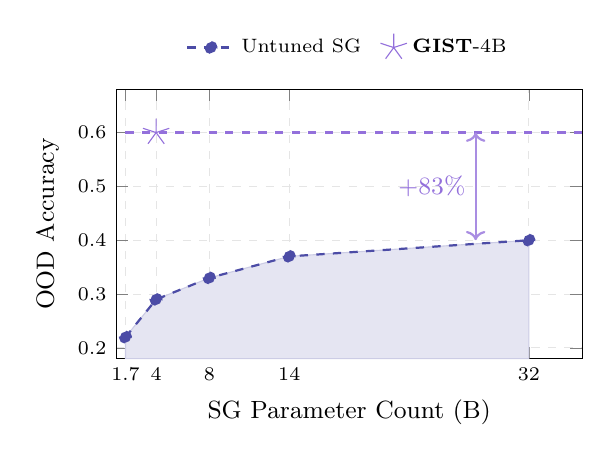
\begin{tikzpicture}
    \begin{axis}[
      width  = 7.5cm,
      height = 5.0cm,
      xlabel = {SG Parameter Count (B)},
      ylabel = {OOD Accuracy},
      xlabel style = {font=\small},
      ylabel style = {font=\small},
      xticklabel style = {font=\scriptsize},
      yticklabel style = {font=\scriptsize},
      xmin = 1.0, xmax = 36,
      ymin = 0.18, ymax = 0.68,
      xtick = {1.7, 4, 8, 14, 32},
      xticklabels = {1.7, 4, 8, 14, 32},
      ytick = {0.2, 0.3, 0.4, 0.5, 0.6},
      grid = major,
      grid style = {gray!20, dashed},
      legend style = {at={(0.5,1.08)}, anchor=south,
                      font=\scriptsize, row sep=0pt,
                      legend columns=2,
                      draw=none, fill=none,
                      /tikz/every even column/.append style={column sep=5pt}},
      clip = false,
    ]
      % shaded region under untuned SG curve
      \addplot[NavyBlue!20, fill=NavyBlue!10, forget plot]
        coordinates {(1.7,0.22)(4,0.29)(8,0.33)(14,0.37)(32,0.40)(32,0.18)(1.7,0.18)}
        -- cycle;
      % untuned SG line
      \addplot[NavyBlue!70, thick, dashed, mark=*, mark size=2pt,
               mark options={fill=NavyBlue!70}]
        coordinates {(1.7,0.22)(4,0.29)(8,0.33)(14,0.37)(32,0.40)};
      \addlegendentry{Untuned SG};
      % horizontal dashed line at GIST-4B level
      \addplot[MediumPurple, thick, dashed, forget plot]
        coordinates {(1.7,0.60)(36,0.60)};
      % GIST-4B star point
      \addplot[MediumPurple, only marks, mark=star, mark size=5pt,
               mark options={fill=MediumPurple}]
        coordinates {(4,0.60)};
      \addlegendentry{\gist{}-4B};
      % annotation arrow placed inside axis to avoid right overflow
      \draw[<->, MediumPurple!80, thick]
        (axis cs:28,0.40) -- (axis cs:28,0.60)
        node[midway, left, font=\small, MediumPurple] {$+$83\%};
    \end{axis}
  \end{tikzpicture}}
  \caption{Scale improves untuned SG gradually; meta-inductive training shifts the curve far more strongly (\gist{}-4B surpasses 32B untuned SG by $+83\%$, AS fixed to Qwen3-4B).}
  \label{fig:scale_sweep_main}
\end{figure}

\paragraph{非单例复制.}
为直接检验 \gist{} 是否改变模型对支持集的利用方式，我们对同批任务分别用
Pre-/Post-\gist{} 的 SG 做 leave-one-out 灵敏度分析：
每次删去一个支持示例后重新生成策略，以余弦相似度衡量策略偏移幅度，
得到每个示例的贡献分布。
对分布计算归一化熵 $H_{\mathrm{ex}}$（越高说明整合越均匀）与峰值贡献 $D_{\mathrm{max}}$（越高说明越依赖单例）。
此外，\texttt{[INDUCTIVE\_RULE]} 段由 GPT-5 盲评归纳质量：
abstraction\_score（是否任务级抽象）与 copying\_score（是否单例复制）。

图~\ref{fig:induction_mechanism}(a) 显示，Post-\gist{} 的 $H_{\mathrm{ex}}$ 从 0.52 升至 0.88，
$D_{\mathrm{max}}$ 从 0.79 降至 0.41，表明 SG 从"锚定单个示例"转向"均匀整合支持集"。
图~\ref{fig:induction_mechanism}(b) 归因热力图进一步揭示：Pre-\gist{} 的规则组件几乎全部
溯源于某一个示例（单列深色），而 Post-\gist{} 的各组件均匀分布于三个示例，
印证了真正的多示例归纳。

% Figure 4 (new): 2-panel induction mechanism
\begin{figure}[t]
  \centering
  %
  % ── Panel (a): leave-one-out bar chart ───────────────────────────
  \begin{minipage}[c]{0.29\columnwidth}
    \centering
    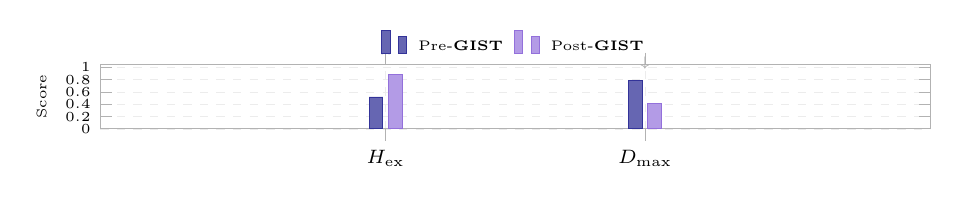
\begin{tikzpicture}
      \begin{axis}[
        ybar, bar width=5pt,
        width=\linewidth, height=2.4cm,
        ymin=0, ymax=1.05,
        ytick={0,0.2,0.4,0.6,0.8,1.0},
        yticklabel style={font=\tiny},
        ylabel={Score},
        ylabel style={font=\tiny},
        xtick={1,2},
        xticklabels={$H_{\mathrm{ex}}$, $D_{\mathrm{max}}$},
        xticklabel style={font=\scriptsize},
        xmin=0.5, xmax=2.5,
        enlarge x limits=0.30,
        axis line style={gray!60, line width=0.4pt},
        tick style={gray!60, line width=0.35pt},
        grid=major, grid style={gray!15, very thin, dashed},
        legend style={at={(0.5,1.02)}, anchor=south, font=\tiny,
                      legend columns=2, draw=none, fill=none,
                      column sep=2pt, inner sep=1pt},
        clip=false,
      ]
        \addplot[fill=NavyBlue!60, draw=NavyBlue!80, line width=0.3pt]
          coordinates {(1,0.52)(2,0.79)};
        \addlegendentry{Pre-\gist{}};
        \addplot[fill=MediumPurple!70, draw=MediumPurple, line width=0.3pt]
          coordinates {(1,0.88)(2,0.41)};
        \addlegendentry{Post-\gist{}};
        \node[font=\tiny, gray!65, anchor=south] at (axis cs:1,0.91) {$\uparrow$};
        \node[font=\tiny, gray!65, anchor=south] at (axis cs:2,0.82) {$\downarrow$};
      \end{axis}
    \end{tikzpicture}\\[2pt]
    {\scriptsize\bfseries(a)}
  \end{minipage}%
  \hspace{0.04\columnwidth}%
  %
  % ── Panel (b): attribution heatmaps ─────────────────────────────
  \begin{minipage}[c]{0.64\columnwidth}
    \centering
    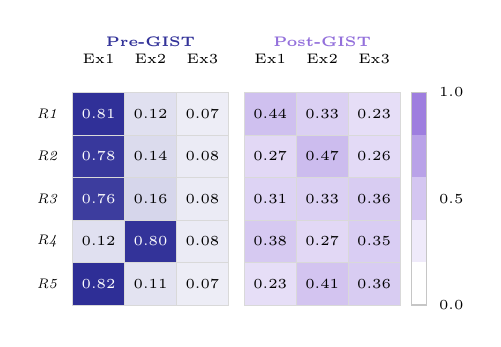
\begin{tikzpicture}[font=\tiny, x=1cm, y=1cm]
      % Layout parameters (all in cm)
      \pgfmathsetmacro{\cw}{0.66}    % cell width
      \pgfmathsetmacro{\ch}{0.54}    % cell height
      \pgfmathsetmacro{\rl}{0.26}    % row-label column
      \pgfmathsetmacro{\hg}{0.20}    % inter-heatmap gap
      % Column x-origins: Pre-GIST
      \pgfmathsetmacro{\pa}{\rl}
      \pgfmathsetmacro{\pb}{\rl+\cw}
      \pgfmathsetmacro{\pc}{\rl+2*\cw}
      % Column x-origins: Post-GIST
      \pgfmathsetmacro{\qa}{\rl+3*\cw+\hg}
      \pgfmathsetmacro{\qb}{\rl+3*\cw+\hg+\cw}
      \pgfmathsetmacro{\qc}{\rl+3*\cw+\hg+2*\cw}
      % Colorbar x-origin
      \pgfmathsetmacro{\cbx}{\rl+6*\cw+\hg+0.14}

      % ── Row labels ──────────────────────────────────────────────
      \node[anchor=east] at ({\pa-0.05},{-0.5*\ch})  {\textit{R1}};
      \node[anchor=east] at ({\pa-0.05},{-1.5*\ch})  {\textit{R2}};
      \node[anchor=east] at ({\pa-0.05},{-2.5*\ch})  {\textit{R3}};
      \node[anchor=east] at ({\pa-0.05},{-3.5*\ch})  {\textit{R4}};
      \node[anchor=east] at ({\pa-0.05},{-4.5*\ch})  {\textit{R5}};

      % ── Pre-GIST header ─────────────────────────────────────────
      \node[font=\tiny\bfseries, NavyBlue!80, anchor=south]
        at ({\pa+1.5*\cw},{0.46}) {Pre-\gist{}};
      \node[anchor=south] at ({\pa+0.5*\cw},{0.24}) {Ex1};
      \node[anchor=south] at ({\pb+0.5*\cw},{0.24}) {Ex2};
      \node[anchor=south] at ({\pc+0.5*\cw},{0.24}) {Ex3};

      % Pre-GIST R1: 0.81 / 0.12 / 0.07
      \fill[NavyBlue!81!white](\pa,0)        rectangle ++(\cw,-\ch);
      \draw[gray!30,very thin](\pa,0)        rectangle ++(\cw,-\ch);
      \node[text=white] at ({\pa+0.5*\cw},{-0.5*\ch}) {0.81};
      \fill[NavyBlue!12!white](\pb,0)        rectangle ++(\cw,-\ch);
      \draw[gray!30,very thin](\pb,0)        rectangle ++(\cw,-\ch);
      \node at ({\pb+0.5*\cw},{-0.5*\ch}) {0.12};
      \fill[NavyBlue!7!white] (\pc,0)        rectangle ++(\cw,-\ch);
      \draw[gray!30,very thin](\pc,0)        rectangle ++(\cw,-\ch);
      \node at ({\pc+0.5*\cw},{-0.5*\ch}) {0.07};

      % Pre-GIST R2: 0.78 / 0.14 / 0.08
      \fill[NavyBlue!78!white](\pa,{-\ch})   rectangle ++(\cw,-\ch);
      \draw[gray!30,very thin](\pa,{-\ch})   rectangle ++(\cw,-\ch);
      \node[text=white] at ({\pa+0.5*\cw},{-1.5*\ch}) {0.78};
      \fill[NavyBlue!14!white](\pb,{-\ch})   rectangle ++(\cw,-\ch);
      \draw[gray!30,very thin](\pb,{-\ch})   rectangle ++(\cw,-\ch);
      \node at ({\pb+0.5*\cw},{-1.5*\ch}) {0.14};
      \fill[NavyBlue!8!white] (\pc,{-\ch})   rectangle ++(\cw,-\ch);
      \draw[gray!30,very thin](\pc,{-\ch})   rectangle ++(\cw,-\ch);
      \node at ({\pc+0.5*\cw},{-1.5*\ch}) {0.08};

      % Pre-GIST R3: 0.76 / 0.16 / 0.08
      \fill[NavyBlue!76!white](\pa,{-2*\ch}) rectangle ++(\cw,-\ch);
      \draw[gray!30,very thin](\pa,{-2*\ch}) rectangle ++(\cw,-\ch);
      \node[text=white] at ({\pa+0.5*\cw},{-2.5*\ch}) {0.76};
      \fill[NavyBlue!16!white](\pb,{-2*\ch}) rectangle ++(\cw,-\ch);
      \draw[gray!30,very thin](\pb,{-2*\ch}) rectangle ++(\cw,-\ch);
      \node at ({\pb+0.5*\cw},{-2.5*\ch}) {0.16};
      \fill[NavyBlue!8!white] (\pc,{-2*\ch}) rectangle ++(\cw,-\ch);
      \draw[gray!30,very thin](\pc,{-2*\ch}) rectangle ++(\cw,-\ch);
      \node at ({\pc+0.5*\cw},{-2.5*\ch}) {0.08};

      % Pre-GIST R4: 0.12 / 0.80 / 0.08
      \fill[NavyBlue!12!white](\pa,{-3*\ch}) rectangle ++(\cw,-\ch);
      \draw[gray!30,very thin](\pa,{-3*\ch}) rectangle ++(\cw,-\ch);
      \node at ({\pa+0.5*\cw},{-3.5*\ch}) {0.12};
      \fill[NavyBlue!80!white](\pb,{-3*\ch}) rectangle ++(\cw,-\ch);
      \draw[gray!30,very thin](\pb,{-3*\ch}) rectangle ++(\cw,-\ch);
      \node[text=white] at ({\pb+0.5*\cw},{-3.5*\ch}) {0.80};
      \fill[NavyBlue!8!white] (\pc,{-3*\ch}) rectangle ++(\cw,-\ch);
      \draw[gray!30,very thin](\pc,{-3*\ch}) rectangle ++(\cw,-\ch);
      \node at ({\pc+0.5*\cw},{-3.5*\ch}) {0.08};

      % Pre-GIST R5: 0.82 / 0.11 / 0.07
      \fill[NavyBlue!82!white](\pa,{-4*\ch}) rectangle ++(\cw,-\ch);
      \draw[gray!30,very thin](\pa,{-4*\ch}) rectangle ++(\cw,-\ch);
      \node[text=white] at ({\pa+0.5*\cw},{-4.5*\ch}) {0.82};
      \fill[NavyBlue!11!white](\pb,{-4*\ch}) rectangle ++(\cw,-\ch);
      \draw[gray!30,very thin](\pb,{-4*\ch}) rectangle ++(\cw,-\ch);
      \node at ({\pb+0.5*\cw},{-4.5*\ch}) {0.11};
      \fill[NavyBlue!7!white] (\pc,{-4*\ch}) rectangle ++(\cw,-\ch);
      \draw[gray!30,very thin](\pc,{-4*\ch}) rectangle ++(\cw,-\ch);
      \node at ({\pc+0.5*\cw},{-4.5*\ch}) {0.07};

      % ── Post-GIST header ────────────────────────────────────────
      \node[font=\tiny\bfseries, MediumPurple, anchor=south]
        at ({\qa+1.5*\cw},{0.46}) {Post-\gist{}};
      \node[anchor=south] at ({\qa+0.5*\cw},{0.24}) {Ex1};
      \node[anchor=south] at ({\qb+0.5*\cw},{0.24}) {Ex2};
      \node[anchor=south] at ({\qc+0.5*\cw},{0.24}) {Ex3};

      % Post-GIST R1: 0.44 / 0.33 / 0.23
      \fill[MediumPurple!44!white](\qa,0)        rectangle ++(\cw,-\ch);
      \draw[gray!30,very thin]    (\qa,0)        rectangle ++(\cw,-\ch);
      \node at ({\qa+0.5*\cw},{-0.5*\ch}) {0.44};
      \fill[MediumPurple!33!white](\qb,0)        rectangle ++(\cw,-\ch);
      \draw[gray!30,very thin]    (\qb,0)        rectangle ++(\cw,-\ch);
      \node at ({\qb+0.5*\cw},{-0.5*\ch}) {0.33};
      \fill[MediumPurple!23!white](\qc,0)        rectangle ++(\cw,-\ch);
      \draw[gray!30,very thin]    (\qc,0)        rectangle ++(\cw,-\ch);
      \node at ({\qc+0.5*\cw},{-0.5*\ch}) {0.23};

      % Post-GIST R2: 0.27 / 0.47 / 0.26
      \fill[MediumPurple!27!white](\qa,{-\ch})   rectangle ++(\cw,-\ch);
      \draw[gray!30,very thin]    (\qa,{-\ch})   rectangle ++(\cw,-\ch);
      \node at ({\qa+0.5*\cw},{-1.5*\ch}) {0.27};
      \fill[MediumPurple!47!white](\qb,{-\ch})   rectangle ++(\cw,-\ch);
      \draw[gray!30,very thin]    (\qb,{-\ch})   rectangle ++(\cw,-\ch);
      \node at ({\qb+0.5*\cw},{-1.5*\ch}) {0.47};
      \fill[MediumPurple!26!white](\qc,{-\ch})   rectangle ++(\cw,-\ch);
      \draw[gray!30,very thin]    (\qc,{-\ch})   rectangle ++(\cw,-\ch);
      \node at ({\qc+0.5*\cw},{-1.5*\ch}) {0.26};

      % Post-GIST R3: 0.31 / 0.33 / 0.36
      \fill[MediumPurple!31!white](\qa,{-2*\ch}) rectangle ++(\cw,-\ch);
      \draw[gray!30,very thin]    (\qa,{-2*\ch}) rectangle ++(\cw,-\ch);
      \node at ({\qa+0.5*\cw},{-2.5*\ch}) {0.31};
      \fill[MediumPurple!33!white](\qb,{-2*\ch}) rectangle ++(\cw,-\ch);
      \draw[gray!30,very thin]    (\qb,{-2*\ch}) rectangle ++(\cw,-\ch);
      \node at ({\qb+0.5*\cw},{-2.5*\ch}) {0.33};
      \fill[MediumPurple!36!white](\qc,{-2*\ch}) rectangle ++(\cw,-\ch);
      \draw[gray!30,very thin]    (\qc,{-2*\ch}) rectangle ++(\cw,-\ch);
      \node at ({\qc+0.5*\cw},{-2.5*\ch}) {0.36};

      % Post-GIST R4: 0.38 / 0.27 / 0.35
      \fill[MediumPurple!38!white](\qa,{-3*\ch}) rectangle ++(\cw,-\ch);
      \draw[gray!30,very thin]    (\qa,{-3*\ch}) rectangle ++(\cw,-\ch);
      \node at ({\qa+0.5*\cw},{-3.5*\ch}) {0.38};
      \fill[MediumPurple!27!white](\qb,{-3*\ch}) rectangle ++(\cw,-\ch);
      \draw[gray!30,very thin]    (\qb,{-3*\ch}) rectangle ++(\cw,-\ch);
      \node at ({\qb+0.5*\cw},{-3.5*\ch}) {0.27};
      \fill[MediumPurple!35!white](\qc,{-3*\ch}) rectangle ++(\cw,-\ch);
      \draw[gray!30,very thin]    (\qc,{-3*\ch}) rectangle ++(\cw,-\ch);
      \node at ({\qc+0.5*\cw},{-3.5*\ch}) {0.35};

      % Post-GIST R5: 0.23 / 0.41 / 0.36
      \fill[MediumPurple!23!white](\qa,{-4*\ch}) rectangle ++(\cw,-\ch);
      \draw[gray!30,very thin]    (\qa,{-4*\ch}) rectangle ++(\cw,-\ch);
      \node at ({\qa+0.5*\cw},{-4.5*\ch}) {0.23};
      \fill[MediumPurple!41!white](\qb,{-4*\ch}) rectangle ++(\cw,-\ch);
      \draw[gray!30,very thin]    (\qb,{-4*\ch}) rectangle ++(\cw,-\ch);
      \node at ({\qb+0.5*\cw},{-4.5*\ch}) {0.41};
      \fill[MediumPurple!36!white](\qc,{-4*\ch}) rectangle ++(\cw,-\ch);
      \draw[gray!30,very thin]    (\qc,{-4*\ch}) rectangle ++(\cw,-\ch);
      \node at ({\qc+0.5*\cw},{-4.5*\ch}) {0.36};

      % ── Colorbar (height = 5*\ch, matching heatmap) ─────────────
      \fill[MediumPurple!90!white] ({\cbx},0)          rectangle ++(0.20,-\ch);
      \fill[MediumPurple!65!white] ({\cbx},{-\ch})      rectangle ++(0.20,-\ch);
      \fill[MediumPurple!40!white] ({\cbx},{-2*\ch})    rectangle ++(0.20,-\ch);
      \fill[MediumPurple!15!white] ({\cbx},{-3*\ch})    rectangle ++(0.20,-\ch);
      \fill[white]                 ({\cbx},{-4*\ch})    rectangle ++(0.20,-\ch);
      \draw[gray!45,thin]          ({\cbx},0)           rectangle ++(0.20,{-5*\ch});
      \node[anchor=west] at ({\cbx+0.23},{0})           {1.0};
      \node[anchor=west] at ({\cbx+0.23},{-2.5*\ch})    {0.5};
      \node[anchor=west] at ({\cbx+0.23},{-5*\ch})      {0.0};

    \end{tikzpicture}\\[2pt]
    {\scriptsize\bfseries(b)}
  \end{minipage}
  \caption{\gist{} shifts SG from single-example copying to integrated
    multi-example induction: \textbf{(a)}~leave-one-out attribution shows
    higher $H_{\mathrm{ex}}$ and lower $D_{\mathrm{max}}$ post-training;
    \textbf{(b)}~rule components trace uniformly to all three support examples
    (Post-\gist{}) rather than collapsing onto one (Pre-\gist{}).}
  \label{fig:induction_mechanism}
\end{figure}

% ============================================================
\subsection{Where Are the Gains Stored?}
\label{sec:internalization}

表~\ref{tab:internalization} 沿两个正交轴分解训练效应：参数是否已更新（训练前/后）× 推理时是否生成策略。
FS $\Delta{=}{+}0.20^*$（$p{<}0.05$）量化纯参数内化——训练后模型在完全不生成策略的条件下 OOD 即显著提升；\gist{}$-$FS$={+}0.06$ 进一步量化推理时显式策略步骤的\emph{额外}贡献，两者互补而非替代。跨格式内化测试表明内化效应与提示格式无关（完整表格见附录~F）。

% Table: Internalization decomposition
\begin{table}[h!]
  \centering
  \fontsize{7.5pt}{8.8pt}\selectfont
  \setlength{\tabcolsep}{3pt}
  \renewcommand{\arraystretch}{1.05}
  \resizebox{\columnwidth}{!}{%
  \begin{tabular}{
    @{}
    >{\raggedright\arraybackslash}p{0.42\columnwidth}
    S[table-format=1.2]
    S[table-format=1.2]
    >{\centering\arraybackslash}p{0.15\columnwidth}
    @{}
  }
    \toprule
    \textbf{Inference Mode} & {\textbf{Pre-train}} & {\textbf{Post-train}} & {$\bm{\Delta}$} \\
    \midrule
    \textbf{0S} (zero-shot, no strategy)    & 0.20 & 0.36 & {$+$0.16} \\
    \textbf{FS} ($K{=}3$, no strategy) $\star$ & 0.34 & 0.54 & {$+$0.20$^{*}$} \\
    \textbf{H-0S} (zero-shot + strategy)    & 0.29 & 0.42 & {$+$0.13} \\
    \textbf{\gist{}} ($K{=}3$ + strategy)  & 0.29 & 0.60 & {$+$0.31} \\
    \midrule
    \multicolumn{3}{@{}l}{\gist{} $-$ FS (both post-training)} & {$+$0.06} \\
    \bottomrule
  \end{tabular}%
  }
  \caption{FS row ($\star$) isolates parameter internalization; \gist{}$-$FS quantifies inference-time strategy gain (Qwen3-4B, OOD accuracy).}
  \label{tab:internalization}
\end{table}

图~\ref{fig:category_radar} 沿六类归纳模式对 Pre-/Post-\gist{} 策略进行打分
（Gemini-3-flash，0--5，归一化后绘制；评分 prompt 见附录~\ref{app:six_modes_prompt}）。
Post-\gist{} 在全部六个维度上均显著超越 Pre-\gist{}：
Procedural（$+1.8$）与 Compositional（$+1.7$）增益最大，
表明 RL 训练的核心效益在于提升策略的算法化能力与规则组合深度；
Constraint-based 与 Schema-induction 各提升约 $+1.7$ 分，
进一步证明 Post-\gist{} 策略能更准确地刻画任务边界与任务族结构。
上述六维认知提升与表~\ref{tab:internalization} 的参数内化分解互补：
归纳能力既编码于参数（$\Delta_{\text{FS}}{=}{+}0.20$），
也体现于推理时策略的整体认知质量。

% Figure 5: six induction modes radar
\begin{figure}[h!]
  \centering
  \resizebox{0.82\columnwidth}{!}{%
    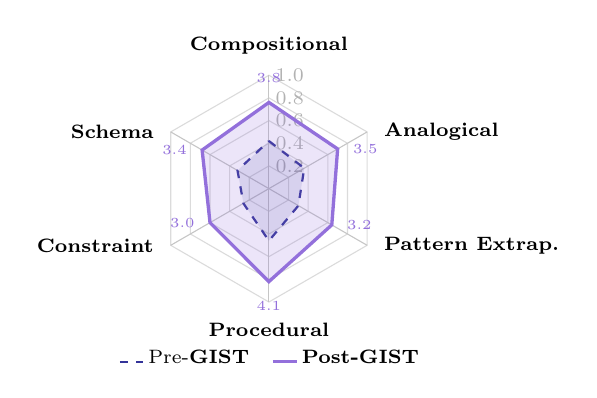
\begin{tikzpicture}[font=\scriptsize, scale=0.72]
      % --- grid: 5 concentric hexagons ---
      \foreach \k in {1,...,5}{
        \pgfmathsetmacro{\R}{0.4*\k}
        \draw[gray!28, thin]
          (0,\R) -- ({\R*0.866},{\R*0.5}) -- ({\R*0.866},{-\R*0.5})
          -- (0,-\R) -- ({-\R*0.866},{-\R*0.5}) -- ({-\R*0.866},{\R*0.5}) -- cycle;
      }
      % 6 radial axes
      \foreach \ang in {90,30,-30,-90,-150,150}{
        \pgfmathsetmacro{\ex}{2.0*cos(\ang)}
        \pgfmathsetmacro{\ey}{2.0*sin(\ang)}
        \draw[gray!45, thin] (0,0) -- (\ex,\ey);
      }
      % scale labels
      \foreach \v/\r in {0.2/0.4, 0.4/0.8, 0.6/1.2, 0.8/1.6, 1.0/2.0}{
        \node[gray!60, anchor=west, inner sep=1pt] at (0.06,\r) {\v};
      }
      % axis labels (six induction modes, clockwise from top)
      \node[font=\scriptsize\bfseries, above]  at (0,    2.20)          {Compositional};
      \node[font=\scriptsize\bfseries, right]  at (1.86, 1.00)          {Analogical};
      \node[font=\scriptsize\bfseries, right]  at (1.86,-1.00)          {Pattern Extrap.};
      \node[font=\scriptsize\bfseries, below]  at (0,   -2.20)          {Procedural};
      \node[font=\scriptsize\bfseries, left]   at (-1.86,-1.00)         {Constraint};
      \node[font=\scriptsize\bfseries, left]   at (-1.86, 1.00)         {Schema};
      % Pre-GIST polygon (normalised scores: .42,.36,.30,.46,.26,.32)
      \draw[NavyBlue!80, thick, dashed, fill=NavyBlue!80, fill opacity=0.12]
        (0,      0.84) --
        ( 0.623, 0.36) --
        ( 0.520,-0.30) --
        (0,     -0.92) --
        (-0.450,-0.26) --
        (-0.554, 0.32) -- cycle;
      % Post-GIST polygon (normalised scores: .76,.70,.64,.82,.60,.68)
      \draw[MediumPurple, very thick, fill=MediumPurple, fill opacity=0.18]
        (0,      1.52) --
        ( 1.212, 0.70) --
        ( 1.109,-0.64) --
        (0,     -1.64) --
        (-1.039,-0.60) --
        (-1.178, 0.68) -- cycle;
      % Post-GIST vertex labels (raw 0-5 scores)
      \node[MediumPurple, font=\tiny, above] at (0,      1.52+0.18)  {3.8};
      \node[MediumPurple, font=\tiny, right] at (1.212+0.10, 0.70)   {3.5};
      \node[MediumPurple, font=\tiny, right] at (1.109+0.10,-0.64)   {3.2};
      \node[MediumPurple, font=\tiny, below] at (0,     -1.64-0.18)  {4.1};
      \node[MediumPurple, font=\tiny, left]  at (-1.039-0.10,-0.60)  {3.0};
      \node[MediumPurple, font=\tiny, left]  at (-1.178-0.10, 0.68)  {3.4};
      % legend
      \node[anchor=north, inner sep=0pt] at (0,-2.80) {%
        \begin{tabular}{@{}c@{\,}l@{\quad}c@{\,}l@{}}
          \tikz\draw[NavyBlue!80, thick, dashed] (0,0.07)--(0.30,0.07); & Pre-\gist{} &
          \tikz\draw[MediumPurple, very thick]   (0,0.07)--(0.30,0.07); & \textbf{Post-\gist{}}
        \end{tabular}%
      };
    \end{tikzpicture}%
  }
  \caption{Six-mode induction scoring (Gemini-3-flash, 0--5, normalised;
    prompt in App.~\ref{app:six_modes_prompt}) reveals that \gist{} training
    lifts all induction dimensions, with Procedural and Compositional
    showing the largest gains ($+1.8$ and $+1.7$ respectively).}
  \label{fig:category_radar}
\end{figure}

% ============================================================
\subsection{How Reusable Are the Learned Strategies?}
\label{sec:reusability}

\paragraph{策略来源决定质量.}
图~\ref{fig:strategy_quality} 使用 GPT-5 作为策略质量裁判，逐项比较 \gist{} 训练后的 Qwen3-4B 与 GPT-5 生成的策略（评分 prompt 见附录~\ref{app:strategy_quality_prompt}）。
在 Correctness 与 Transferability 上，Qwen3-4B 分别以 52\%/49\% 的胜率高于 GPT-5 的 46\%/31\%，说明跨任务 RL 学到的策略更偏向任务规律抽象与迁移。
GPT-5 在 Executability（57\% vs.\ 40\%）与 Conciseness（39\% vs.\ 31\%）上占优，表明闭源强模型仍具有更好的步骤表达与压缩能力；但 Transferability 的 20\% 平局和 Qwen3-4B 的领先共同显示，\gist{} 优化的核心收益在于可复用的归纳策略，而非表面语言质量。

% Figure 6: strategy quality
\begin{figure}[H]
  \centering
  \resizebox{0.98\columnwidth}{!}{%
  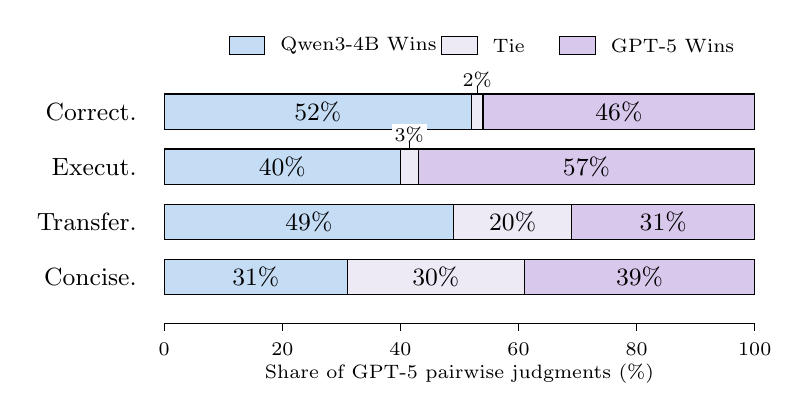
\begin{tikzpicture}[x=0.075cm,y=0.70cm]
    \tikzset{
      qseg/.style={draw=black, line width=0.45pt},
      qlabel/.style={font=\small, anchor=east},
      qpct/.style={font=\small},
      qtiny/.style={font=\scriptsize, fill=white, inner sep=1pt}
    }

    % Legend
    \node[qseg, fill=qualityQwen, minimum width=0.45cm, minimum height=0.17cm] at (14,4.30) {};
    \node[font=\scriptsize, anchor=west] at (18,4.30) {Qwen3-4B Wins};
    \node[qseg, fill=qualityTie, minimum width=0.45cm, minimum height=0.17cm] at (50,4.30) {};
    \node[font=\scriptsize, anchor=west] at (54,4.30) {Tie};
    \node[qseg, fill=qualityGPT, minimum width=0.45cm, minimum height=0.17cm] at (70,4.30) {};
    \node[font=\scriptsize, anchor=west] at (74,4.30) {GPT-5 Wins};

    % Correctness: Qwen 52, Tie 2, GPT-5 46
    \node[qlabel] at (-3,3.10) {Correct.};
    \draw[qseg, fill=qualityQwen] (0,2.78) rectangle (52,3.42);
    \draw[qseg, fill=qualityTie] (52,2.78) rectangle (54,3.42);
    \draw[qseg, fill=qualityGPT] (54,2.78) rectangle (100,3.42);
    \node[qpct] at (26,3.10) {52\%};
    \node[qtiny] at (53,3.68) {2\%};
    \draw[thin] (53,3.42) -- (53,3.57);
    \node[qpct] at (77,3.10) {46\%};

    % Executability: Qwen 40, Tie 3, GPT-5 57
    \node[qlabel] at (-3,2.10) {Execut.};
    \draw[qseg, fill=qualityQwen] (0,1.78) rectangle (40,2.42);
    \draw[qseg, fill=qualityTie] (40,1.78) rectangle (43,2.42);
    \draw[qseg, fill=qualityGPT] (43,1.78) rectangle (100,2.42);
    \node[qpct] at (20,2.10) {40\%};
    \node[qtiny] at (41.5,2.68) {3\%};
    \draw[thin] (41.5,2.42) -- (41.5,2.57);
    \node[qpct] at (71.5,2.10) {57\%};

    % Transferability: Qwen 49, Tie 20, GPT-5 31
    \node[qlabel] at (-3,1.10) {Transfer.};
    \draw[qseg, fill=qualityQwen] (0,0.78) rectangle (49,1.42);
    \draw[qseg, fill=qualityTie] (49,0.78) rectangle (69,1.42);
    \draw[qseg, fill=qualityGPT] (69,0.78) rectangle (100,1.42);
    \node[qpct] at (24.5,1.10) {49\%};
    \node[qpct] at (59,1.10) {20\%};
    \node[qpct] at (84.5,1.10) {31\%};

    % Conciseness: Qwen 31, Tie 30, GPT-5 39
    \node[qlabel] at (-3,0.10) {Concise.};
    \draw[qseg, fill=qualityQwen] (0,-0.22) rectangle (31,0.42);
    \draw[qseg, fill=qualityTie] (31,-0.22) rectangle (61,0.42);
    \draw[qseg, fill=qualityGPT] (61,-0.22) rectangle (100,0.42);
    \node[qpct] at (15.5,0.10) {31\%};
    \node[qpct] at (46,0.10) {30\%};
    \node[qpct] at (80.5,0.10) {39\%};

    % Axis
    \draw[black, line width=0.4pt] (0,-0.75) -- (100,-0.75);
    \foreach \x/\lab in {0/0,20/20,40/40,60/60,80/80,100/100} {
      \draw[black, line width=0.35pt] (\x,-0.75) -- (\x,-0.88);
      \node[font=\scriptsize, anchor=north] at (\x,-0.92) {\lab};
    }
    \node[font=\scriptsize] at (50,-1.65) {Share of GPT-5 pairwise judgments (\%)};
  \end{tikzpicture}%
  }
  \caption{Strategy quality analysis using GPT-5 as evaluator. Each bar reports the share of pairwise judgments favoring the \gist{}-trained Qwen3-4B strategy, a tie, or the GPT-5-generated strategy on the corresponding dimension.}
  \label{fig:strategy_quality}
\end{figure}

\paragraph{求解器可迁移性.}
固定 SG-4B，将 AS 替换为更强的 AS-14B/32B，OOD 准确率单调提升（表~\ref{tab:solver_transfer}；AS-32B vs.\ AS-8B: $+0.08$），证明同一自然语言策略是与求解器无关的可组合指令，部署时可免训练升级 \as{}。

% Table 5: Solver transferability
\begin{table}[h!]
  \centering
  \fontsize{8pt}{10pt}\selectfont
  \setlength{\tabcolsep}{6pt}
  \renewcommand{\arraystretch}{1.1}
  \begin{tabular}{@{}ll S[table-format=1.2] S[table-format=+1.2]@{}}
    \toprule
    \textbf{SG} & \textbf{AS} & {\textbf{OOD Acc}$\uparrow$} & {$\bm{\Delta}$ vs AS-4B} \\
    \midrule
    SG-4B & AS-8B  & 0.60 & {—} \\
    SG-4B & AS-14B & 0.64 & {$+$0.04} \\
    SG-4B & AS-32B & 0.68 & {$+$0.08} \\
    \bottomrule
  \end{tabular}
  \caption{Same SG-4B strategy improves monotonically with stronger executors (no retraining needed).}
  \label{tab:solver_transfer}
\end{table}

\paragraph{质性案例.}
表~\ref{tab:case_study} 展示一个 ICL 失败而 \gist{} 成功的典型 OOD 实例（选取标准：(a) ICL 作答错误；(b) \gist{} 作答正确；(c) \texttt{[INDUCTIVE\_RULE]} 体现跨实例抽象；(d) 任务来自 OOD 集）。
\texttt{[INDUCTIVE\_RULE]} 段使归纳步骤显式化，实现 ICL 不具备的可解释、可纠错推理。
失败案例（附录~G，$\kappa{=}{\cdash}$）主要源于 \texttt{[INDUCTIVE\_RULE]} 段规则提取不完整，而非执行器错误。

% Table 6: Case study
\begin{table}[h!]
  \centering
  \small
  \setlength{\tabcolsep}{5pt}
  \renewcommand{\arraystretch}{1.12}
  \begin{tabular}{p{0.12\columnwidth} p{0.80\columnwidth}}
    \toprule
    \multicolumn{2}{>{\raggedright\arraybackslash}p{0.94\columnwidth}}{%
      \textbf{Task}: [OOD task---to be selected from actual model outputs per criteria (a)--(d)]%
    } \\
    \midrule
    \textbf{ICL} & [ICL output---fails on this instance] \\
    \midrule
    \textbf{\gist{}} &
      \textbf{[INDUCTIVE\_RULE]} [Abstract rule induced from support set] \newline
      \textbf{[APPLICABILITY]} [Scope conditions] \newline
      \textbf{[TASK\_PROCEDURE]} [Step-by-step execution] \newline
      \textbf{Answer}: [Correct] \\
    \bottomrule
  \end{tabular}
  \caption{Qualitative comparison on an OOD task. ICL relies on surface pattern matching and fails; \gist{} induces an abstract rule and applies it step by step, yielding interpretable reasoning. App.~G provides a failure case analysis.}
  \label{tab:case_study}
\end{table}


% ============================================================
\section{Related Work}
\label{sec:related}

\textbf{元学习与上下文学习.} 经典元学习（MAML~\citep{finn2017maml}、Prototypical Networks~\citep{snell2017prototypical}）优化快速适配，但难以产出可显式复用的自然语言策略。MetaICL~\citep{min2022metaicl} 证明 ICL 可训练，而 Wang et al.~\citep{wang2024icl_ood} 与 de Wynter~\citep{dewynter2025icl} 指出其仍受限于假设空间检索与示例利用率。\gist{} 以跨任务 RL 将归纳习惯固化为行为先验，直接针对上述隐式匹配瓶颈。

\textbf{强化学习增强推理.} CoT~\citep{wei2022cot}、STaR~\citep{zelikman2022star}、Quiet-STaR~\citep{zelikman2024quietstar}、DeepSeek-R1~\citep{deepseek2025r1} 及交互式学习~\citep{klissarov2026interactive} 主要优化对象层“如何解”，而非从示范中提炼可迁移策略的元层归纳。\gist{} 将 RL 对准策略生成，并以 EIR$\times$ICR 联合奖励显式塑造该层能力。

\textbf{逐任务提示优化.} APE~\citep{zhou2023ape}、OPRO~\citep{yang2024opro}、PromptBreeder~\citep{fernando2023promptbreeder}、GEPA~\citep{agrawal2025gepa} 在单任务上搜索提示，成本高且成果难跨任务迁移。\gist{} 则一次训练将 learn-to-induce 写入参数，对新 OOD 任务单次前向即可生成策略。

% ============================================================
\section{Conclusion}
\label{sec:conclusion}

本文提出 \gist{}，通过跨任务强化学习将元归纳习惯训练为 LLM 的稳定认知行为。双层解耦框架将策略归纳（\sg{}，RL 训练）与策略执行（\as{}，冻结）分离，以执行准确率为唯一奖励，无需策略层面的人工标注。难度自适应增量奖励有效缓解了难度耦合问题，$M$ 次采样稳定化显著降低了 RL 训练方差。在三类评测集上的实验表明，训练后的 4B \sg{} 相对于 few-shot ICL 基线在 BIG-Bench OOD 任务上最高提升 $+84\%$，在三种异构骨架上均取得统计显著的正增益。核心发现是：元归纳习惯是与参数规模正交的认知维度，必须通过有目标的 RL 训练显式培养，而非期望随模型规模自然涌现。

% ============================================================
\section{Limitations}
\label{sec:limitations}

\paragraph{Training cost.}
每个训练 episode 需要 $G \times M = 32$ 次 \as{} 前向推理，计算开销约为标准 SFT 的 32 倍。尽管可通过批处理并行化，但仍对 GPU 资源有较高要求。

\paragraph{Solver coupling.}
\sg{} 的策略在训练过程中被优化为适配特定 \as{}（Qwen3-8B）。尽管 §\ref{sec:analysis} 的 Solver Transferability 实验表明策略可迁移至更强的求解器，但切换至架构差异显著的 \as{} 时仍可能出现策略-求解器分布偏移。策略-求解器联合优化是未来的重要方向。

\paragraph{Benchmark coverage.}
当前评测集以英文任务为主；元归纳能力在多语言和多模态场景下的泛化性尚待验证。BBH 与训练集存在部分任务类型重叠，更严格的 OOD 协议有待构建。

\paragraph{Reward reliability.}
增量奖励依赖基线准确率 $b$ 的离线历史估计；在任务分布变化较大时，$b$ 的估计可能存在偏差，影响奖励方向。

\paragraph{Backbone-dependent gain magnitude.}
\gist{} achieves statistically significant OOD gains across all three open backbones, but the magnitude varies strongly ($+84\%$/$+24\%$/$+9\%$ for Qwen3-4B/Gemma-3-4B/LLaMA-3.1-8B), likely reflecting differences in pre-training task coverage and instruction-tuning quality.
Reducing this backbone dependency is an important direction for future work.

\paragraph{BIG-Bench intra-distribution similarity.}
The $N$ training tasks and the BIG-Bench OOD evaluation tasks share the same task taxonomy, introducing potential meta-distribution similarity.
MATH500, StrategyQA, and ReClor serve as cross-dataset stress tests, but their current results are pending and will be incorporated in the camera-ready version to strengthen the cross-domain generalisation claim.

\paragraph{Single-run training stability.}
All results are from a single training run.
The reported cluster bootstrap CIs quantify evaluation uncertainty but do not capture training-seed variance.
Multi-run stability analysis is deferred to future work.

% ============================================================
\bibliography{references}

% ============================================================
\appendix

\section{Training Algorithm and Implementation Details}
\label{app:training}

\subsection{Models, Evaluation Protocols, and Baselines}
\label{app:models}

\textbf{骨架模型.}
为避免正文重复，本节集中列出所有模型、推理协议与基线方法。
\gist{} 主要在开源主干 \textbf{Qwen3-4B/8B}~\citep{yang2025qwen3technicalreport}、\textbf{LLaMA-3.1-8B}~\citep{dubey2024llama3}、\textbf{Gemma-3-4B}~\citep{gemmateam2025gemma3} 上评测。
闭源 API（\textbf{Gemini-3-flash}~\citep{google2025gemini3flash}、\textbf{GPT-5}~\citep{openai2025gpt54}）不参与微调，仅作为推理时参考上界。
数据过滤评分与 SFT 示范生成使用 Gemini-3-flash 作为教师模型。

\textbf{推理协议.}
\textbf{0S} 表示 zero-shot 直接作答；
\textbf{H-0S} 表示 zero-shot strategy-then-answer，两次调用同一骨架；
\textbf{FS} 表示 $K$-shot 直接 ICL 作答；
\textbf{H-FS} 表示 $K$-shot strategy-then-answer，无 RL 训练；
\textbf{\gist{}} 表示经过跨任务 GRPO 训练后的 strategy-then-answer 模式。
因此 FS/H-FS/0S/H-0S 是施加在模型骨架上的 evaluation protocols，而非独立模型基线。

\textbf{数值格式.}
本文所有表格中的准确率数值均以百分数形式呈现（例如，``45.00'' 表示 45.00\%），$\Delta$\% 列亦为相对变化的百分点数值。

\textbf{基线方法.}
\textbf{MetaICL}~\citep{min2022metaicl} 用于比较同等训练成本下、无显式策略归纳目标的跨任务元训练。
\textbf{OPRO}~\citep{yang2024opro} 与 \textbf{GEPA}~\citep{agrawal2025gepa} 用于比较逐任务推理时 prompt 优化；GEPA 采用 Gemini-3-flash 作为优化器、Qwen3-4B 作为执行器，运行 4 次反思式迭代。
默认超参数：$G{=}8$，$M{=}4$，$K{=}3$，$\beta{=}0.5$；硬件 8$\times$A800；完整训练配置见下节。

\subsection{Hyperparameters}

\begin{table}[H]
  \centering
  \small
  \setlength{\tabcolsep}{5pt}
  \renewcommand{\arraystretch}{1.12}
  \resizebox{\columnwidth}{!}{%
  \begin{tabular}{ll}
    \toprule
    \textbf{Hyperparameter} & \textbf{Value} \\
    \midrule
    \multicolumn{2}{l}{\textit{Model configuration}} \\
    Strategy Generator (\sg{}) & Qwen3-4B (trainable) \\
    Answer Solver (\as{})       & Qwen3-8B (frozen, non-thinking mode) \\
    Hardware                    & 8$\times$A800 (80\,GB) \\
    Training time               & ${\sim}$12--24 h (one full \gist{} run) \\
    \midrule
    \multicolumn{2}{l}{\textit{Training hyperparameters}} \\
    Rollout count $G$             & 8 \\
    Evaluation samples $M$        & 4 \\
    Few-shot shots $K$            & 3 \\
    Learning rate                 & $1\times10^{-6}$ (AdamW) \\
    Max generation length         & 4{,}096 tokens \\
    Training data                 & ${\sim}$20K samples \\
    Batch size                    & {\cdash} \\
    Total training steps          & {\cdash} \\
    \midrule
    \multicolumn{2}{l}{\textit{Reward parameters}} \\
    Asymm.\ weight $\alpha^+$ (positive gain) & 0.7 \\
    Asymm.\ weight $\alpha^-$ (negative gain) & 0.3 \\
    ICR amplification $\beta$     & 0.5 \\
    Log-smoothing constant $k$    & 10 \\
    Lower-bound cutoff $\varepsilon$  & $10^{-4}$ \\
    Baseline EMA decay $\gamma$   & 0.9 \\
    Format penalty $\lambda_{\text{fmt}}$ & 1.0 \\
    \bottomrule
  \end{tabular}%
  }
  \caption{Hyperparameters for \gist{} training.}
  \label{tab:hyperparams}
\end{table}

\FloatBarrier

\subsection{EIR: Difficulty-Adaptive Normalizer}
\label{app:eir_normalizer}

归一化分母 $c(b_\tau)$ 在式~\eqref{eq:eir_raw} 中定义为
\begin{equation}
  c(b_\tau) = \max\!\bigl(b_\tau^{\,\alpha}(1-b_\tau)^{1-\alpha},\; \varepsilon\bigr)
  \label{eq:c_btau}
\end{equation}
其中 $\alpha$ 根据 $\delta_i$ 的符号选取，$\varepsilon = 10^{-4}$ 为下界截断以防数值不稳定。

\paragraph{数学性质.}
函数 $b^\alpha(1-b)^{1-\alpha}$（$b \in [0,1]$）是参数为 $(\alpha+1, 2-\alpha)$ 的 Beta 分布的非归一化概率密度，其在 $b = \alpha$ 处取唯一极大值。当 $b_\tau = \alpha$ 时 $c(b_\tau)$ 最大，$g_\text{raw} = |\delta_i|/c(b_\tau)$ 取最小；当 $b_\tau$ 远离 $\alpha$（极易 $b_\tau \to 1$ 或极难 $b_\tau \to 0$）时，$c(b_\tau)$ 收缩，$g_\text{raw}$ 放大——对极端难度任务的偏移赋予更高权重，回应 R1。

\paragraph{非对称 $\alpha$ 的作用.}
$\alpha^+ = 0.7 > \alpha^- = 0.3$ 实现两项不同的难度校准：
\begin{itemize}[leftmargin=*, nosep]
  \item \textbf{正向（$\delta_i \geq 0$，$\alpha = \alpha^+$）}：$c(b_\tau)$ 在 $b_\tau = 0.7$ 处峰值，使中高难度任务的改进获得自然基准，极难任务（$b_\tau \ll 0.7$）的提升被放大。
  \item \textbf{负向（$\delta_i < 0$，$\alpha = \alpha^-$）}：$c(b_\tau)$ 在 $b_\tau = 0.3$ 处峰值，高基线任务（$b_\tau \gg 0.3$）退步时 $c(b_\tau)$ 更小，惩罚力度系统性增大；低基线任务退步时 $c(b_\tau)$ 相对较大，保留训练早期的探索多样性。
\end{itemize}

\paragraph{消融.}
移除非对称设计（令 $\alpha^+ = \alpha^- = 0.5$）时，高基线任务的退步惩罚减弱，导致高资源任务上 OOD 迁移下降约 1.3\%（见表~\ref{tab:ablation} EIR-sym 行）。$\varepsilon$ 的具体值对最终性能不敏感（$10^{-5}$ 至 $10^{-3}$ 范围内变化小于 0.2\%）。

\FloatBarrier
\subsection{Two-Stage Training Pipeline}

\textbf{Stage 0 (SFT warm-up):} A small set of teacher-constructed demonstrations is used to fine-tune $\pi_{\sg{}}$ to produce format-compliant strategies.
This stage typically converges in a few hundred steps and serves solely to bootstrap format adherence above 90\% before RL begins.
\textbf{Stage 1 (Inductive alignment):} The full joint reward $R_i$ (Eq.~\eqref{eq:total_reward}) is used; $\pi_{\sg{}}$ is trained to produce strategies that are simultaneously accurate, difficulty-aware, and internally decisive. Format-invalid strategies are skipped (see format gating below).
Task sampling is stratified-uniform across all task types; each episode selects one task type at random.

\paragraph{Format gating.} A binary format check validates whether all required schema sections are present and structurally valid. Format-invalid strategies receive a fixed penalty $R_i = -\lambda_\text{fmt}$ (with $\lambda_\text{fmt} = 1.0$) and are not passed to \as{} for execution; EIR and ICR are not computed for them. This fixed-penalty design (as opposed to simply excluding invalid strategies from GRPO) ensures that \sg{} is actively discouraged from generating malformed outputs: excluding would remove the gradient signal entirely, whereas the fixed penalty provides a consistent negative signal that regularizes the output format throughout training.

\subsection{Training Algorithm}

\begin{algorithm}[H]
\caption{\gist{} Training (Phase 2: Inductive Alignment)}
\label{alg:mist}
\begin{algorithmic}[1]
\Require Task distribution $P(\mathcal{T})$; SFT-initialized $\pi_{\sg{}}^{(0)}$; frozen \as{}; baseline buffer $\{b_\tau\}$ (init from SFT inference); EMA decay $\gamma$; total steps $N$
\For{step $= 1, \ldots, N$}
  \State Sample $\tau \sim P(\mathcal{T})$; retrieve baseline $b_\tau$
  \State Sample $\mathcal{D}_\text{spt}^{(\tau)} = \{(x_i,y_i)\}_{i=1}^K$ and $\mathcal{D}_\text{qry}^{(\tau)}$: $M$ queries $\{(x_m, y^*_m)\}_{m=1}^M$
  \State Sample $G$ strategies: $\{s_g\}_{g=1}^G \sim \pi_{\sg{}}(\cdot \mid \mathcal{D}_\text{spt}^{(\tau)})$
  \For{each $s_g$}
    \If{$R_\text{fmt}(s_g) = 0$} $R_g \leftarrow -\lambda_\text{fmt}$; \textbf{skip} to reward collection \EndIf
    \State $A_\text{curr} \leftarrow \tfrac{1}{M}\sum_{m=1}^M \mathbb{1}[\as{}(s_g, x_m) = y^*_m]$,\quad $\delta \leftarrow A_\text{curr} - b_\tau$ \Comment{proxy utility}
    \State Compute $g_\text{raw}$ via Eq.~\eqref{eq:eir_raw} with asymmetric $\alpha$
    \State $R_{\text{EIR},g} \leftarrow \operatorname{sign}(\delta) \cdot \ln(1 + k\,g_\text{raw})$ \Comment{Eq.~\eqref{eq:eir}}
    \State $R_{\text{ICR},g} \leftarrow \tfrac{1}{M}\sum_{m=1}^{M}\exp\!\Bigl(\tfrac{1}{T_m}\sum_{t=1}^{T_m}\log P_\text{AS}\!\bigl(y_t^{(m)} \mid y_{<t}^{(m)},\, s_g,\, x_m\bigr)\Bigr)$ \Comment{Eq.~\eqref{eq:icr}}
    \State $R_g \leftarrow R_{\text{EIR},g} \cdot (1 + \beta \cdot R_{\text{ICR},g})$ \Comment{Eq.~\eqref{eq:total_reward}}
  \EndFor
  \State $\hat{A}_g \leftarrow (R_g - \tfrac{1}{G}\sum_{g'} R_{g'}) \;/\; (\operatorname{std}(\{R_{g''}\}) + \epsilon)$ \Comment{GRPO advantage~\citep{shao2024grpo}}
  \State Update $\pi_{\sg{}}$ via GRPO using $\{\hat{A}_g\}$; \as{} remains frozen
  \State Update baseline buffer: $b_\tau \leftarrow (1-\gamma)\,b_\tau + \gamma\,A_\text{curr}$
\EndFor
\end{algorithmic}
\end{algorithm}

\section{Full Strategy Schema and Format Comparison}
\label{app:schema}

本附录首先对比四种策略格式的 prompt 设计与典型输出（§\ref{app:four_formats}），随后给出 \mist{} 半结构化格式的完整规范与跨领域样例（§\ref{app:schema_spec}）。

% ──────────────────────────────────────────────────────────────
\subsection{四种策略格式对比}
\label{app:four_formats}

我们以 BIG-Bench Navigate 任务（网格坐标追踪，判断是否回到起点）为统一场景，对比四种格式在 prompt 设计、典型 \sg{} 输出及关键缺陷上的差异。这四种格式对应表~\ref{tab:ablation_format} 的四行，沿"结构化程度"轴排列：Free-form（无）$\to$ CoT-style（隐式）$\to$ Semi-structured（\mist{}，推荐）$\to$ Rigid-schema（过度）。

\paragraph{① Free-form（无结构）.}
\textbf{Prompt 设计}：
\begin{quote}\small\ttfamily
Based on the following examples, generate a strategy
to solve this type of problem.

[few-shot examples]

Strategy:
\end{quote}
\noindent\textbf{典型 \sg{} 输出}：
\begin{quote}\small\ttfamily
Track coordinates. North +y, South -y, East +x, West -x.
Check if (x,y) = (0,0) at end.
\end{quote}
\noindent\textbf{关键缺陷}：输出完全无约束——上例仅两句话，下一次可能是十句段落。\as{} 面对长度与结构不一致的 prompt，token 级对数概率基准无法跨样本对比，ICR 不可测。\sg{} 倾向于针对具体示例转述，缺乏可验证的任务族级归纳规律，OOD 泛化最弱。

\paragraph{② CoT-style（隐式结构）.}
\textbf{Prompt 设计}：
\begin{quote}\small\ttfamily
Based on the following examples, analyze the pattern
and generate a step-by-step strategy for solving this
type of problem. Think carefully and reason step by step.

[few-shot examples]

Strategy:
\end{quote}
\noindent\textbf{典型 \sg{} 输出}：
\begin{quote}\small\ttfamily
Let me analyze the examples:
- Example 1: coordinates update with each direction...
- Example 2: same pattern confirmed...

General approach:
1. Initialize position (0,0)
2. Parse each instruction...
3. Check if final position is origin

This should work for similar grid navigation problems,
though diagonal movements might need special handling.
\end{quote}
\noindent\textbf{关键缺陷}：有推理步骤但无强制节划分——归纳规律（``coordinates update''）与执行步骤（编号列表）混写，边界条件（``diagonal movements''）散落在段末，无固定位置。\as{} 面对不同长度、不同结构的 prompt，\texttt{[INDUCTIVE\_RULE]} anchor 消失，对数概率基准不一致，ICR 中等；OOD 迁移因归纳边界未被显式管理而弱于半结构化。

\paragraph{③ Semi-structured / \mist{}（推荐）.}
\textbf{Prompt 设计}：
\begin{quote}\small\ttfamily
Based on the following examples, generate a strategy
using EXACTLY the following sections:
[INDUCTIVE\_RULE] / [TASK\_PROCEDURE] / [TRANSFER\_SCOPE]

[few-shot examples]

Strategy:
\end{quote}
\noindent\textbf{典型 \sg{} 输出}（参见 §\ref{app:schema_spec} 完整样例）：
\begin{quote}\small\ttfamily
[INDUCTIVE\_RULE]
坐标更新规则：北(+y), 南(-y), 东(+x), 西(-x)。
判断终点是否为原点(0,0)。

[TASK\_PROCEDURE]
1. 初始化 (x,y)=(0,0)
2. 逐条解析指令，提取方向与步数
3. 更新坐标
4. 判断 (x,y)==(0,0)，输出 Yes/No

[TRANSFER\_SCOPE]
触发：题目包含方向性移动指令，询问是否回到起点。
不适用：含对角移动或条件分支指令时需扩展步骤2。
\end{quote}
\noindent\textbf{优势}：三节分工明确，\as{} 始终面对固定节头，token 级对数概率基准一致，ICR 可测；\texttt{INDUCTIVE\_RULE} 强制显式归纳，\texttt{TRANSFER\_SCOPE} 显式管理边界，OOD 最强。

\paragraph{④ Rigid-schema（过度结构化，JSON 输出）.}
\textbf{Prompt 设计}：
\begin{quote}\small\ttfamily
Based on the following examples, output a strategy
as a JSON object with keys: "rule", "steps",
"applicable\_when", "not\_applicable".

[few-shot examples]

Strategy (JSON):
\end{quote}
\noindent\textbf{典型 \sg{} 输出}：
\begin{quote}\small\ttfamily
\{
  "rule": "north=+y, south=-y, east=+x, west=-x",
  "steps": ["init (0,0)", "parse", "update", "check"],
  "applicable\_when": "grid navigation",
  "not\_applicable": "diagonal movement"
\}
\end{quote}
\noindent\textbf{关键缺陷}：花括号、引号、冒号等 JSON 格式 token 大量占据 \as{} 解码的概率分布，干扰策略语义与 \as{} 语言理解先验的对齐（Prior Compatibility，§\ref{sec:arch}）；步骤被压缩为简短字符串（``parse''、``update''），丧失可执行性；ICR 反而低于半结构化，验证自然语言半结构的接口兼容性优势。

% ──────────────────────────────────────────────────────────────
\subsection{半结构化格式完整规范}
\label{app:schema_spec}

\mist{} 的半结构化策略 $s$ 要求 \sg{} 生成固定节名的文本块。完整规范如下。

\subsection{三节强制格式}

每条策略须包含三个强制性节，以节名行（形如 \texttt{[SECTION\_NAME]}）为分隔符：

\begin{itemize}[leftmargin=*, itemsep=2pt]
  \item \textbf{\texttt{[INDUCTIVE\_RULE]}}：陈述从 $K$ 个示例中提炼的核心归纳规律，规律须为任务族级别（跨实例通用），而非针对特定示例的描述。要求：(i) 规律须可对照示例验证；(ii) 规律表述不针对具体实例，而是对整类任务成立。（边界条件与不适用情形统一归入 \texttt{TRANSFER\_SCOPE}，此节不重复列出。）
  \item \textbf{\texttt{[TASK\_PROCEDURE]}}：3—6 条面向当前任务族的操作步骤，以编号列表形式呈现。要求：(i) 每步须为可执行动作，而非描述性总结；(ii) 步骤须覆盖完整求解路径（输入解析→中间推理→输出格式化）。
  \item \textbf{\texttt{[TRANSFER\_SCOPE]}}：策略适用范围的完整规格，统一管理所有边界信息。要求：(i) 须显式列举触发条件（何时套用本策略）；(ii) 须给出至少一个"不适用"情形；(iii) 若 \texttt{INDUCTIVE\_RULE} 中的规律有已知例外，在此列出。
\end{itemize}

格式违规判定：\texttt{INDUCTIVE\_RULE}、\texttt{TASK\_PROCEDURE}、\texttt{TRANSFER\_SCOPE} 任意一节缺失、节名拼写错误，或节内容为空，均视为格式不合规，该策略获得固定惩罚 $R_i = -\lambda_\text{fmt}$（$\lambda_\text{fmt} = 1.0$），不传入 \as{} 执行。

\subsection{策略样例：BIG-Bench Navigate 任务}

以下为 Navigate 任务（网格坐标追踪）的完整策略样例，展示三节格式的标准写法。

\begin{quote}\small\ttfamily
[INDUCTIVE\_RULE]

从示例可归纳：每条指令形如"向\{方向\}走\{步数\}步"，坐标更新规则为：
北(+y), 南(-y), 东(+x), 西(-x)。最终判断目标点是否在原点(0,0)。

[TASK\_PROCEDURE]

1. 初始化坐标 (x, y) = (0, 0)。
2. 逐条解析指令，提取方向与步数。
3. 按规则更新坐标：北→y+=步数，南→y-=步数，东→x+=步数，西→x-=步数。
4. 遍历全部指令后，判断 (x, y) 是否等于 (0, 0)。
5. 若是则输出"Yes"，否则输出"No"。

[TRANSFER\_SCOPE]

触发条件：题目包含一系列方向性移动指令，询问是否回到起点。
应用方式：直接套用上述坐标追踪步骤，无需额外推断。
不适用情形：(1) 若题目含对角移动，则本规律不适用；
            (2) 若指令包含条件分支（如"若…则向北走"），需在步骤 2 中增加条件判断逻辑。
\end{quote}

\subsection{策略样例：BBH Word Sorting 任务}

以下为 Word Sorting（词汇排序）任务样例，展示跨领域适用性。

\begin{quote}\small\ttfamily
[INDUCTIVE\_RULE]

从示例归纳：任务为将给定单词列表按字母序（忽略大小写）排列。
关键规律：(1) 比较首字母，相同则递归比较后续字母；
(2) 数字字符在字母之前；特殊字符遵循 ASCII 序。

[TASK\_PROCEDURE]

1. 将所有单词统一转为小写以便比较。
2. 对单词列表应用字母序排序（逐字符比较）。
3. 若两词前缀完全相同，较短词排在前面。
4. 按排序结果输出，以逗号分隔。

[TRANSFER\_SCOPE]

触发条件：给定无序单词列表，要求按字母序输出。
应用方式：直接套用步骤 1—4。
不适用情形：(1) 若要求按词频或语义相关性排序，则需替换步骤 2 的排序准则；
            (2) 含空格的词组需整体视为排序单元，步骤 1 需相应调整。
\end{quote}

% ============================================================
% ============================================================
\subsection{Training Dynamics: General-Unit Co-rise}
\label{app:strategy_evolution}

随 EIR+ICR 训练推进，策略文本中通用可迁移单元的比例与 OOD 准确率同步上升（图~\ref{fig:strategy_evolution_app}），
印证联合奖励驱动的是真正的元归纳泛化（标注 rubric 见附录~\ref{app:general_units_rubric}）。
完整训练配置见附录~\ref{app:training}。

% Figure moved from main text §4.1
\begin{figure}[H]
  \centering
  \resizebox{\columnwidth}{!}{%
  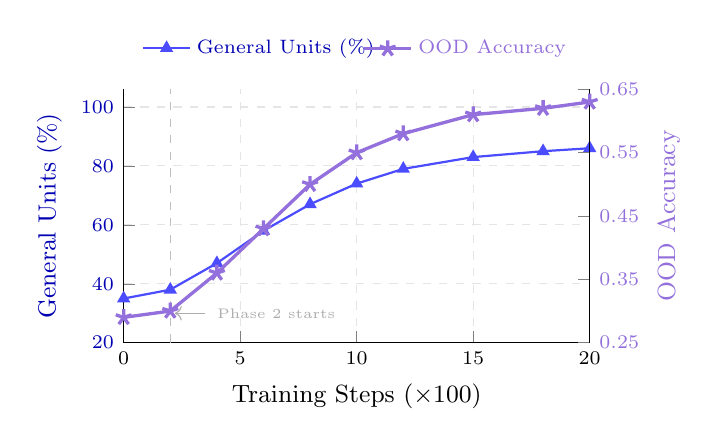
\begin{tikzpicture}
    %% Left axis: General Units (%)
    \begin{axis}[
      name          = ax1,
      xlabel        = {Training Steps ($\times$100)},
      ylabel        = {General Units (\%)},
      ylabel style  = {color=blue!70!black, font=\small},
      yticklabel style = {color=blue!70!black, font=\scriptsize},
      xticklabel style = {font=\scriptsize},
      xlabel style  = {font=\small},
      xmin = 0,   xmax = 20,
      ymin = 20,  ymax = 106,
      ytick = {20, 40, 60, 80, 100},
      xtick = {0, 5, 10, 15, 20},
      width  = 7.5cm,
      height = 4.8cm,
      axis y line* = left,
      axis x line* = bottom,
      grid = major,
      grid style = {gray!20, dashed},
      legend style = {at={(0.02,1.08)}, anchor=south west,
                      font=\scriptsize, row sep=0pt,
                      draw=none, fill=none},
      clip = false,
    ]
      \addplot[blue!70, thick, mark=triangle*, mark size=2pt,
               mark options={fill=blue!70}]
        coordinates {
          (0,35)(2,38)(4,47)(6,58)(8,67)(10,74)(12,79)(15,83)(18,85)(20,86)
        };
      \addlegendentry{\textcolor{blue!70!black}{General Units (\%)}};
      \draw[gray!50, dashed, thin] (axis cs:2,20) -- (axis cs:2,106);
      \draw[->, gray!65, thin] (axis cs:3.5,30) -- (axis cs:2.2,30);
      \node[gray!65, font=\tiny, anchor=west] at (axis cs:3.6,30) {Phase 2 starts};
    \end{axis}
    %% Right axis: OOD Accuracy (overlaid)
    \begin{axis}[
      name          = ax2,
      ylabel        = {OOD Accuracy},
      ylabel style  = {color=MediumPurple, font=\small},
      yticklabel style = {color=MediumPurple, font=\scriptsize},
      xmin = 0,   xmax = 20,
      ymin = 0.25, ymax = 0.65,
      ytick = {0.25, 0.35, 0.45, 0.55, 0.65},
      axis y line* = right,
      axis x line  = none,
      width  = 7.5cm,
      height = 4.8cm,
      legend style = {at={(0.98,1.08)}, anchor=south east,
                      font=\scriptsize, row sep=0pt,
                      draw=none, fill=none},
      clip = false,
    ]
      \addplot[MediumPurple, very thick, mark=star, mark size=3pt,
               mark options={fill=MediumPurple}]
        coordinates {
          (0,0.29)(2,0.30)(4,0.36)(6,0.43)(8,0.50)(10,0.55)(12,0.58)(15,0.61)(18,0.62)(20,0.63)
        };
      \addlegendentry{\textcolor{MediumPurple}{OOD Accuracy}};
    \end{axis}
  \end{tikzpicture}}
  \caption{General-unit proportion and OOD accuracy co-rise during \gist{} training,
           indicating EIR+ICR drives meta-inductive generalisation
           (moved from main text; see also \S\ref{sec:attribution}).}
  \label{fig:strategy_evolution_app}
\end{figure}

% ============================================================
\section{General Units Annotation Rubric}
\label{app:general_units_rubric}

图~\ref{fig:general_units_prompt} 给出用于量化策略文本中"通用单元（General Units）"比例的标注 prompt。
每条策略文本由 Gemini-3-flash 按命题（句子或子句）逐条标注三个二元属性，并组合为四类标签；
\textbf{General Units (\%)} 定义为 T 类与 G 类单元数之和占总单元数的比例。
两轮独立标注的一致率以 Cohen's $\kappa$ 报告（$\kappa{=}{\cdash}$）。

\begin{figure*}[t]
  \centering
  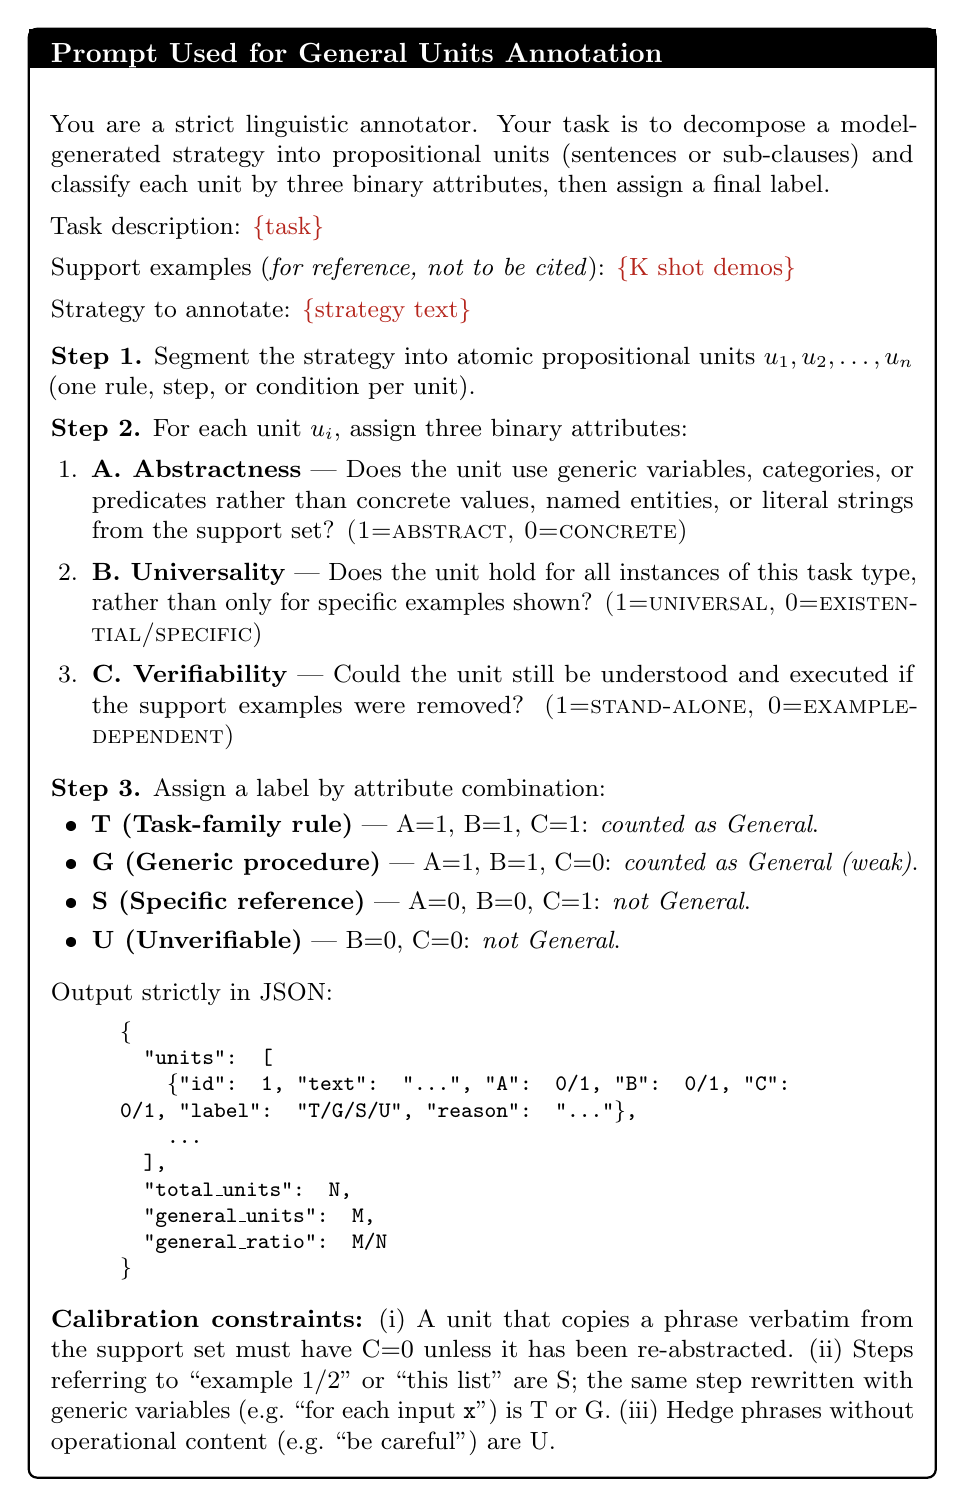
\begin{tikzpicture}
    \node[draw=black, line width=0.8pt, rounded corners=3pt, inner sep=0pt] {%
      \begin{minipage}{0.95\textwidth}
        {\setlength{\fboxsep}{0pt}
        \noindent\colorbox{black}{\makebox[\linewidth][l]{%
          \rule{0pt}{2.8ex}\hspace{8pt}\color{white}\bfseries
          Prompt Used for General Units Annotation}}}
        \vspace{6pt}

        \noindent\hspace{8pt}\begin{minipage}{\dimexpr\linewidth-16pt\relax}
        \small
        You are a strict linguistic annotator. Your task is to decompose a model-generated strategy into propositional units (sentences or sub-clauses) and classify each unit by three binary attributes, then assign a final label.

        \vspace{4pt}
        \noindent Task description: \textcolor{BrickRed}{\{task\}}

        \vspace{4pt}
        \noindent Support examples (\textit{for reference, not to be cited}): \textcolor{BrickRed}{\{K shot demos\}}

        \vspace{4pt}
        \noindent Strategy to annotate: \textcolor{BrickRed}{\{strategy text\}}

        \vspace{6pt}
        \noindent \textbf{Step 1.} Segment the strategy into atomic propositional units $u_1, u_2, \ldots, u_n$ (one rule, step, or condition per unit).

        \vspace{4pt}
        \noindent \textbf{Step 2.} For each unit $u_i$, assign three binary attributes:

        \begin{enumerate}[leftmargin=1.6em, itemsep=2pt, topsep=2pt]
          \item \textbf{A. Abstractness} --- Does the unit use generic variables, categories, or predicates rather than concrete values, named entities, or literal strings from the support set? \textsc{(1=abstract, 0=concrete)}
          \item \textbf{B. Universality} --- Does the unit hold for all instances of this task type, rather than only for specific examples shown? \textsc{(1=universal, 0=existential/specific)}
          \item \textbf{C. Verifiability} --- Could the unit still be understood and executed if the support examples were removed? \textsc{(1=stand-alone, 0=example-dependent)}
        \end{enumerate}

        \vspace{4pt}
        \noindent \textbf{Step 3.} Assign a label by attribute combination:
        \begin{itemize}[leftmargin=1.6em, itemsep=1pt, topsep=2pt]
          \item \textbf{T (Task-family rule)} --- A{=}1, B{=}1, C{=}1: \textit{counted as General}.
          \item \textbf{G (Generic procedure)} --- A{=}1, B{=}1, C{=}0: \textit{counted as General (weak)}.
          \item \textbf{S (Specific reference)} --- A{=}0, B{=}0, C{=}1: \textit{not General}.
          \item \textbf{U (Unverifiable)} --- B{=}0, C{=}0: \textit{not General}.
        \end{itemize}

        \vspace{6pt}
        \noindent Output strictly in JSON:
        \begin{quote}
        \ttfamily\footnotesize
        \{\\
        \hspace*{1em}"units": [\\
        \hspace*{2em}\{"id": 1, "text": "...", "A": 0/1, "B": 0/1, "C": 0/1, "label": "T/G/S/U", "reason": "..."\},\\
        \hspace*{2em}\ldots\\
        \hspace*{1em}],\\
        \hspace*{1em}"total\_units": N,\\
        \hspace*{1em}"general\_units": M,\\
        \hspace*{1em}"general\_ratio": M/N\\
        \}
        \end{quote}

        \vspace{4pt}
        \noindent \textbf{Calibration constraints:}
        (i) A unit that copies a phrase verbatim from the support set must have C{=}0 unless it has been re-abstracted.
        (ii) Steps referring to ``example 1/2'' or ``this list'' are S; the same step rewritten with generic variables (e.g.\ ``for each input \texttt{x}'') is T or G.
        (iii) Hedge phrases without operational content (e.g.\ ``be careful'') are U.
        \end{minipage}
        \vspace{8pt}
      \end{minipage}%
    };
  \end{tikzpicture}
  \caption{Prompt used for General Units annotation. T and G labels jointly count as General Units; S and U do not.}
  \label{fig:general_units_prompt}
\end{figure*}

% ============================================================
\section{Six Induction Modes Scoring Prompt}
\label{app:six_modes_prompt}

图~\ref{fig:six_modes_prompt} 给出 Gemini-3-flash 对策略文本沿六类归纳模式进行 0--5 分逐项打分的 prompt。
六模式的理论基础来自经典归纳推理分类~\citep{holland1989induction}，对应 \gist{} 策略中的不同认知功能：
Compositional 与 Procedural 评估 \texttt{[TASK\_PROCEDURE]} 的组合与算法化能力；
Analogical 与 Pattern Extrapolation 评估 \texttt{[INDUCTIVE\_RULE]} 的结构抽象与外推能力；
Constraint-based 与 Schema 评估 \texttt{[TRANSFER\_SCOPE]} 的边界与任务族识别能力。

\begin{figure*}[t]
  \centering
  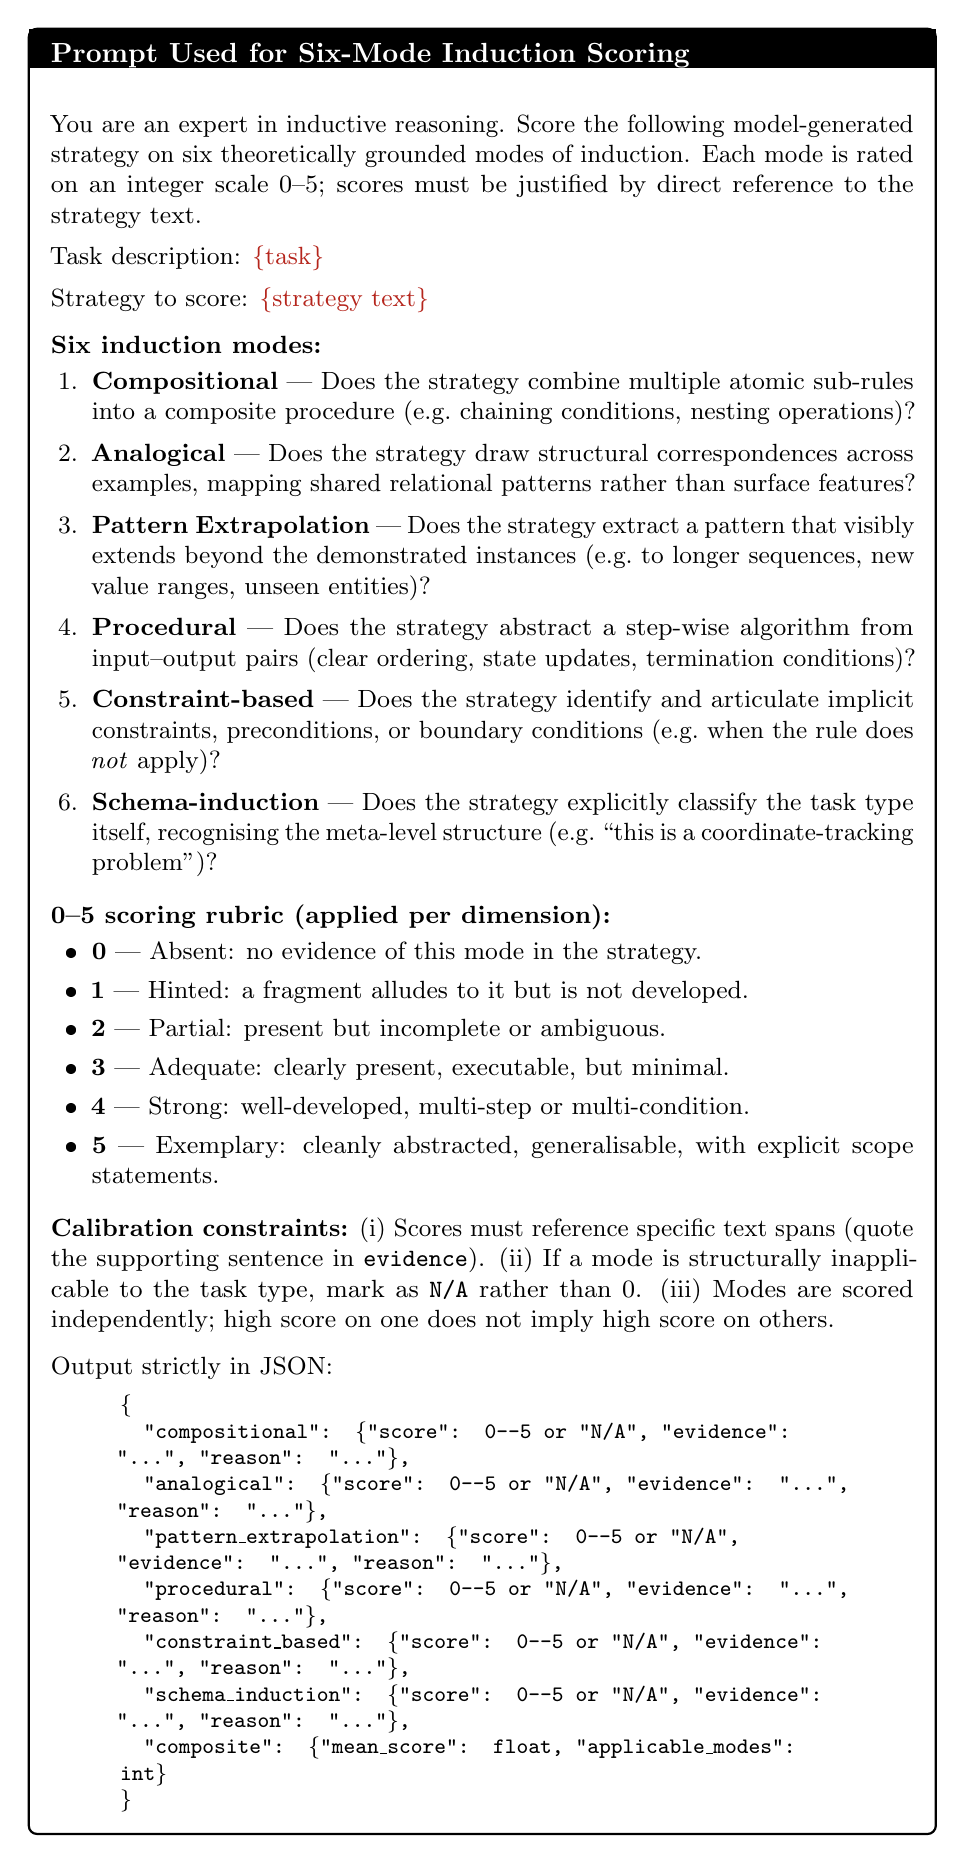
\begin{tikzpicture}
    \node[draw=black, line width=0.8pt, rounded corners=3pt, inner sep=0pt] {%
      \begin{minipage}{0.95\textwidth}
        {\setlength{\fboxsep}{0pt}
        \noindent\colorbox{black}{\makebox[\linewidth][l]{%
          \rule{0pt}{2.8ex}\hspace{8pt}\color{white}\bfseries
          Prompt Used for Six-Mode Induction Scoring}}}
        \vspace{6pt}

        \noindent\hspace{8pt}\begin{minipage}{\dimexpr\linewidth-16pt\relax}
        \small
        You are an expert in inductive reasoning. Score the following model-generated strategy on six theoretically grounded modes of induction. Each mode is rated on an integer scale 0--5; scores must be justified by direct reference to the strategy text.

        \vspace{4pt}
        \noindent Task description: \textcolor{BrickRed}{\{task\}}

        \vspace{4pt}
        \noindent Strategy to score: \textcolor{BrickRed}{\{strategy text\}}

        \vspace{6pt}
        \noindent \textbf{Six induction modes:}
        \begin{enumerate}[leftmargin=1.6em, itemsep=2pt, topsep=2pt]
          \item \textbf{Compositional} --- Does the strategy combine multiple atomic sub-rules into a composite procedure (e.g.\ chaining conditions, nesting operations)?
          \item \textbf{Analogical} --- Does the strategy draw structural correspondences across examples, mapping shared relational patterns rather than surface features?
          \item \textbf{Pattern Extrapolation} --- Does the strategy extract a pattern that visibly extends beyond the demonstrated instances (e.g.\ to longer sequences, new value ranges, unseen entities)?
          \item \textbf{Procedural} --- Does the strategy abstract a step-wise algorithm from input--output pairs (clear ordering, state updates, termination conditions)?
          \item \textbf{Constraint-based} --- Does the strategy identify and articulate implicit constraints, preconditions, or boundary conditions (e.g.\ when the rule does \emph{not} apply)?
          \item \textbf{Schema-induction} --- Does the strategy explicitly classify the task type itself, recognising the meta-level structure (e.g.\ ``this is a coordinate-tracking problem'')?
        \end{enumerate}

        \vspace{6pt}
        \noindent \textbf{0--5 scoring rubric (applied per dimension):}
        \begin{itemize}[leftmargin=1.6em, itemsep=1pt, topsep=2pt]
          \item \textbf{0} --- Absent: no evidence of this mode in the strategy.
          \item \textbf{1} --- Hinted: a fragment alludes to it but is not developed.
          \item \textbf{2} --- Partial: present but incomplete or ambiguous.
          \item \textbf{3} --- Adequate: clearly present, executable, but minimal.
          \item \textbf{4} --- Strong: well-developed, multi-step or multi-condition.
          \item \textbf{5} --- Exemplary: cleanly abstracted, generalisable, with explicit scope statements.
        \end{itemize}

        \vspace{6pt}
        \noindent \textbf{Calibration constraints:}
        (i) Scores must reference specific text spans (quote the supporting sentence in \texttt{evidence}).
        (ii) If a mode is structurally inapplicable to the task type, mark as \texttt{N/A} rather than 0.
        (iii) Modes are scored independently; high score on one does not imply high score on others.

        \vspace{6pt}
        \noindent Output strictly in JSON:
        \begin{quote}
        \ttfamily\footnotesize
        \{\\
        \hspace*{1em}"compositional":   \{"score": 0--5 or "N/A", "evidence": "...", "reason": "..."\},\\
        \hspace*{1em}"analogical":      \{"score": 0--5 or "N/A", "evidence": "...", "reason": "..."\},\\
        \hspace*{1em}"pattern\_extrapolation": \{"score": 0--5 or "N/A", "evidence": "...", "reason": "..."\},\\
        \hspace*{1em}"procedural":      \{"score": 0--5 or "N/A", "evidence": "...", "reason": "..."\},\\
        \hspace*{1em}"constraint\_based": \{"score": 0--5 or "N/A", "evidence": "...", "reason": "..."\},\\
        \hspace*{1em}"schema\_induction": \{"score": 0--5 or "N/A", "evidence": "...", "reason": "..."\},\\
        \hspace*{1em}"composite":        \{"mean\_score": float, "applicable\_modes": int\}\\
        \}
        \end{quote}
        \end{minipage}
        \vspace{8pt}
      \end{minipage}%
    };
  \end{tikzpicture}
  \caption{Prompt used for six-mode induction scoring. Each strategy receives an independent 0--5 score per mode; the composite is the mean over applicable modes (N/A modes excluded from averaging).}
  \label{fig:six_modes_prompt}
\end{figure*}

% ============================================================
\section{Sensitivity Analysis}
\label{app:sensitivity}

Table~\ref{tab:hparam_study} reports hyperparameter sensitivity for $K$, $\beta$, and $\alpha$ on Qwen3-4B; $^\star$ marks the default configuration used in all main-text experiments.

\begin{table}[H]
  \centering
  \small
  \setlength{\tabcolsep}{5pt}
  \renewcommand{\arraystretch}{0.90}
  \resizebox{\columnwidth}{!}{%
  \begin{tabular}{l c S[table-format=1.2] S[table-format=1.2] S[table-format=1.2]}
    \toprule
    \textbf{Parameter} & \textbf{Value} &
    {\textbf{ID}$\uparrow$} & {\textbf{BBH}$\uparrow$} & {\textbf{OOD}$\uparrow$} \\
    \midrule
    \multirow{4}{*}{$K$ (shots)}
      & 0              & {\cdash} & {\cdash} & {\cdash} \\
      & 1              & {\cdash} & {\cdash} & {\cdash} \\
      & $3^{\star}$    & 0.46     & 0.78     & 0.59     \\
      & 5              & {\cdash} & {\cdash} & {\cdash} \\
    \midrule
    \multirow{4}{*}{$\beta$ (ICR weight)}
      & 0              & {\cdash} & {\cdash} & {\cdash} \\
      & 0.2            & {\cdash} & {\cdash} & {\cdash} \\
      & $0.5^{\star}$  & 0.65     & 0.78     & 0.60     \\
      & 0.7            & {\cdash} & {\cdash} & {\cdash} \\
    \midrule
    \multirow{2}{*}{$\alpha$ (EIR asym.)}
      & sym.\ $0.5/0.5$           & {\cdash} & {\cdash} & {\cdash} \\
      & asym.\ $0.7/0.3^{\star}$  & 0.65     & 0.78     & 0.60     \\
    \bottomrule
  \end{tabular}%
  }
  \caption{Hyperparameter sensitivity on Qwen3-4B ($^\star$: default).
    \textbf{$K$}: unlike ICL (saturates at $K{=}2$), \gist{} continues to benefit from additional shots.
    \textbf{$\beta$}: effective over $[0.2, 0.5]$; $\beta{=}0$ degrades to EIR-only.
    \textbf{$\alpha$}: asymmetric EIR weighting outperforms symmetric, stabilising GRPO on hard tasks.}
  \label{tab:hparam_study}
\end{table}

\paragraph{Shot count $K$.}
Unlike standard ICL (which saturates at $K{=}2$), \gist{} continues to benefit from more shots---additional examples provide richer contrast for the \texttt{INDUCTIVE\_RULE} section.
At $K{=}0$, \gist{} still generates effective strategies, confirming that meta-inductive priors are encoded as parametric knowledge.

\paragraph{ICR amplification $\beta$.}
$\beta{=}0$ degrades to EIR-only and significantly decreases ID performance; $\beta{=}0.5$ is optimal.
Results are relatively stable over $[0.2, 0.5]$, indicating that the gain is structural rather than fine-tuning-sensitive.

\paragraph{EIR asymmetry $\alpha$.}
Asymmetric weighting $(\alpha^+, \alpha^-)=(0.7, 0.3)$ gives stronger positive incentive while applying a gentler penalty on negative gains, preventing GRPO from over-suppressing exploration on hard tasks.

% ============================================================
% ============================================================
\section{Per-Task-Type OOD Accuracy by Strategy Source}
\label{app:strategy_source}

表~\ref{tab:strategy_source} 固定执行器为 Qwen3-4B，按策略来源对比五类 OOD 任务的准确率（\%）。

\begin{table}[H]
  \centering
  \setlength{\tabcolsep}{5pt}
  \renewcommand{\arraystretch}{1.1}
  \fontsize{8pt}{10pt}\selectfont
  \resizebox{\columnwidth}{!}{%
  \begin{tabular}{@{}l c c r c@{}}
    \toprule
    \textbf{Task Type} &
    \multicolumn{1}{c}{\makecell{\textbf{Gem.-F}\\FS $\backslash$ H-FS}} &
    \multicolumn{1}{c}{\makecell{\textbf{GPT-5}\\FS $\backslash$ H-FS}} &
    \multicolumn{1}{c}{\textbf{Avg.}} &
    \multicolumn{1}{c}{\makecell{\textbf{Qw3-4B (\gist{})}\\\small($\Delta$ vs.\ Avg.)}} \\
    \midrule
    \quad Ctx.Param.Conf.
      & $75.00\,{\backslash}\,65.00$
      & $70.00\,{\backslash}\,65.00$
      & 68.75
      & \textbf{90.00}\,{\small\textcolor{BrickRed}{(+21.25)}} \\
    \quad VitaminC
      & $85.00\,{\backslash}\,80.00$
      & $65.00\,{\backslash}\,40.00$
      & 67.50
      & 78.33\,{\small\textcolor{BrickRed}{(+10.83)}} \\
    \quad Elem.Math
      & $99.00\,{\backslash}\,89.00$
      & $95.00\,{\backslash}\,75.00$
      & 89.50
      & 97.67\,{\small\textcolor{BrickRed}{(+8.17)}} \\
    \quad Track.Shuf.
      & $100.00\,{\backslash}\,91.67$
      & $85.00\,{\backslash}\,90.00$
      & 91.67
      & 99.44\,{\small\textcolor{BrickRed}{(+7.77)}} \\
    \quad Bool.Expr.
      & $90.00\,{\backslash}\,95.00$
      & $100.00\,{\backslash}\,85.00$
      & 92.50
      & 98.33\,{\small\textcolor{BrickRed}{(+5.83)}} \\
    \bottomrule
  \end{tabular}%
  }
  \caption{OOD accuracy (\%) by strategy source, executor fixed to Qwen3-4B \as{}.
    \textbf{Gem.-F}: Gemini-3-flash (closed-source).
    Each column shows FS (top) $\backslash$ H-FS (bottom).
    \textbf{Avg.}: mean of the four baseline values; $\Delta$: \gist{} vs.\ Avg., sorted descending.}
  \label{tab:strategy_source}
\end{table}

% ============================================================
\section{Strategy Quality Evaluation Prompt}
\label{app:strategy_quality_prompt}

Figure~\ref{fig:strategy_quality_prompt} gives the GPT-5 prompt used to compare strategies generated by the \gist{}-trained Qwen3-4B and GPT-5.
The model identities are provided as Model A and Model B in the prompt, and GPT-5 returns dimension-level preferences and reasons in JSON format.

\begin{figure*}[t]
  \centering
  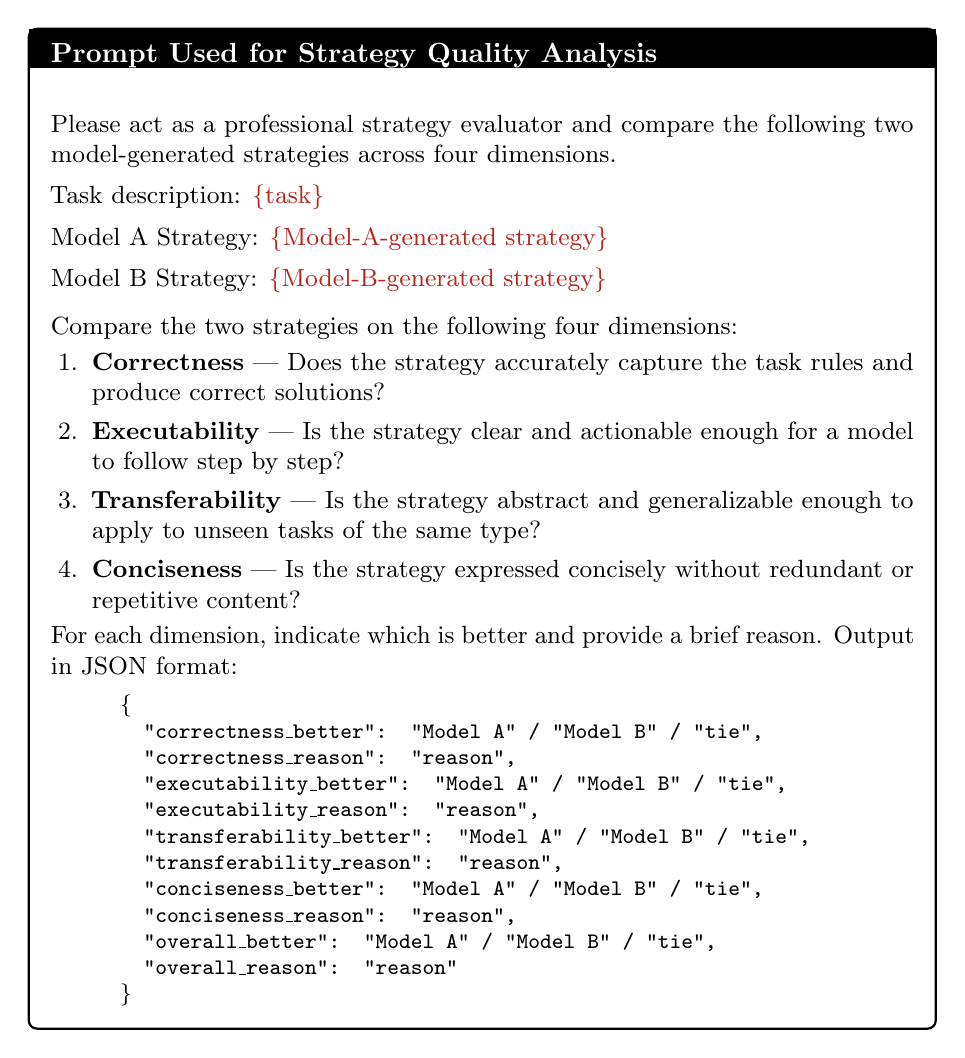
\begin{tikzpicture}
    \node[draw=black, line width=0.8pt, rounded corners=3pt, inner sep=0pt] {%
      \begin{minipage}{0.95\textwidth}
        {\setlength{\fboxsep}{0pt}
        \noindent\colorbox{black}{\makebox[\linewidth][l]{%
          \rule{0pt}{2.8ex}\hspace{8pt}\color{white}\bfseries
          Prompt Used for Strategy Quality Analysis}}}
        \vspace{6pt}

        \noindent\hspace{8pt}\begin{minipage}{\dimexpr\linewidth-16pt\relax}
        \small
        Please act as a professional strategy evaluator and compare the following two model-generated strategies across four dimensions.

        \vspace{4pt}
        \noindent Task description: \textcolor{BrickRed}{\{task\}}

        \vspace{4pt}
        \noindent Model A Strategy: \textcolor{BrickRed}{\{Model-A-generated strategy\}}

        \vspace{4pt}
        \noindent Model B Strategy: \textcolor{BrickRed}{\{Model-B-generated strategy\}}

        \vspace{6pt}
        \noindent Compare the two strategies on the following four dimensions:
        \begin{enumerate}[leftmargin=1.6em, itemsep=1pt, topsep=2pt]
          \item \textbf{Correctness} --- Does the strategy accurately capture the task rules and produce correct solutions?
          \item \textbf{Executability} --- Is the strategy clear and actionable enough for a model to follow step by step?
          \item \textbf{Transferability} --- Is the strategy abstract and generalizable enough to apply to unseen tasks of the same type?
          \item \textbf{Conciseness} --- Is the strategy expressed concisely without redundant or repetitive content?
        \end{enumerate}

        \noindent For each dimension, indicate which is better and provide a brief reason. Output in JSON format:
        \begin{quote}
        \ttfamily\footnotesize
        \{\\
        \hspace*{1em}"correctness\_better": "Model A" / "Model B" / "tie",\\
        \hspace*{1em}"correctness\_reason": "reason",\\
        \hspace*{1em}"executability\_better": "Model A" / "Model B" / "tie",\\
        \hspace*{1em}"executability\_reason": "reason",\\
        \hspace*{1em}"transferability\_better": "Model A" / "Model B" / "tie",\\
        \hspace*{1em}"transferability\_reason": "reason",\\
        \hspace*{1em}"conciseness\_better": "Model A" / "Model B" / "tie",\\
        \hspace*{1em}"conciseness\_reason": "reason",\\
        \hspace*{1em}"overall\_better": "Model A" / "Model B" / "tie",\\
        \hspace*{1em}"overall\_reason": "reason"\\
        \}
        \end{quote}
        \end{minipage}
        \vspace{8pt}
      \end{minipage}%
    };
  \end{tikzpicture}
  \caption{Prompt used for strategy quality analysis.}
  \label{fig:strategy_quality_prompt}
\end{figure*}

% ============================================================
\section{Task-Level ID/OOD Partition}
\label{app:ood_partition}

Full task-level ID/OOD partition table to be provided upon data finalisation.
The partition ensures (i) strict task-ID disjointness between ID and OOD sets, (ii) OOD subtasks preferentially selected from the training-set-sparse categories, and (iii) independent verification by two annotators ($\kappa{=}{\cdash}$).

% ============================================================
\section{Sample Efficiency and Few-Shot Utilization}
\label{app:efficiency}

% Figure: data efficiency
\begin{figure}[H]
  \centering
  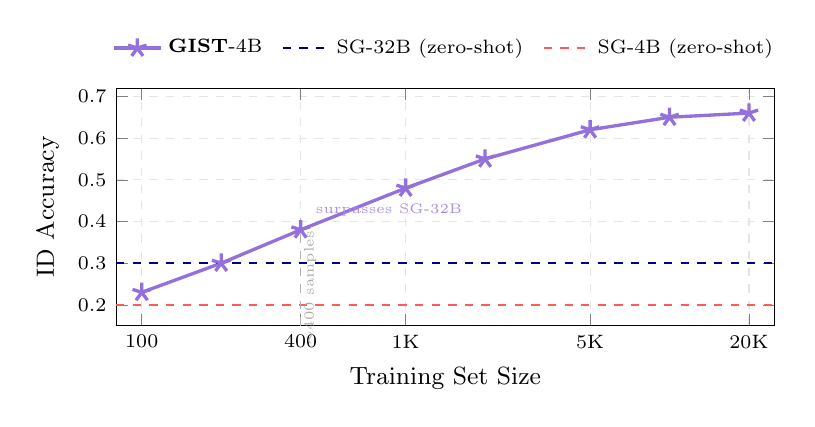
\begin{tikzpicture}
  \begin{axis}[
    xlabel        = {Training Set Size},
    ylabel        = {ID Accuracy},
    xmode         = log,
    log basis x   = 10,
    xtick         = {100, 400, 1000, 5000, 20000},
    xticklabels   = {100, 400, 1K, 5K, 20K},
    xticklabel style = {font=\scriptsize},
    yticklabel style = {font=\scriptsize},
    xlabel style  = {font=\small},
    ylabel style  = {font=\small},
    xmin = 80,    xmax = 25000,
    ymin = 0.15,  ymax = 0.72,
    ytick = {0.2, 0.3, 0.4, 0.5, 0.6, 0.7},
    width  = 0.82\columnwidth,
    height = 4.6cm,
    legend style  = {at={(0.5,1.08)}, anchor=south,
                     font=\scriptsize, row sep=0pt,
                     legend columns=3,
                     draw=none, fill=none,
                     /tikz/every even column/.append style={column sep=5pt}},
    grid          = major,
    grid style    = {gray!20, dashed},
    clip          = false,
  ]
    \addplot[MediumPurple, very thick, mark=star, mark size=3.5pt,
             mark options={fill=MediumPurple}]
      coordinates {
        (100,0.23)(200,0.30)(400,0.38)(1000,0.48)(2000,0.55)
        (5000,0.62)(10000,0.65)(20000,0.66)
      };
    \addlegendentry{\textbf{\gist{}}-4B};
    \addplot[NavyBlue, dashed, thick]
      coordinates {(80,0.30)(25000,0.30)};
    \addlegendentry{SG-32B (zero-shot)};
    \addplot[red!65, dashed, thick]
      coordinates {(80,0.20)(25000,0.20)};
    \addlegendentry{SG-4B (zero-shot)};
    \draw[gray!60, dashed, thin] (axis cs:400,0.15) -- (axis cs:400,0.42);
    \node[gray!65, font=\tiny, rotate=90, anchor=south]
      at (axis cs:500, 0.24) {${\sim}$400 samples};
    \node[MediumPurple!80, font=\tiny, anchor=south west]
      at (axis cs:420, 0.39) {surpasses SG-32B};
  \end{axis}
  \end{tikzpicture}
  \caption{\gist{}-4B ID accuracy vs.\ training set size.
    Only ${\sim}$400 samples suffice to surpass zero-shot SG-32B (0.30),
    demonstrating that EIR+ICR provides dense signal even with scarce data.}
  \label{fig:data_efficiency}
\end{figure}

\gist{}-4B surpasses SG-32B with only ${\sim}$400 training samples, exhibiting a steep early learning curve before plateauing beyond ${\sim}$5K samples.
This suggests the performance ceiling is limited by reward coverage quality and task distribution breadth rather than raw data volume.

% Figure: few-shot utilization
\begin{figure}[H]
  \centering
  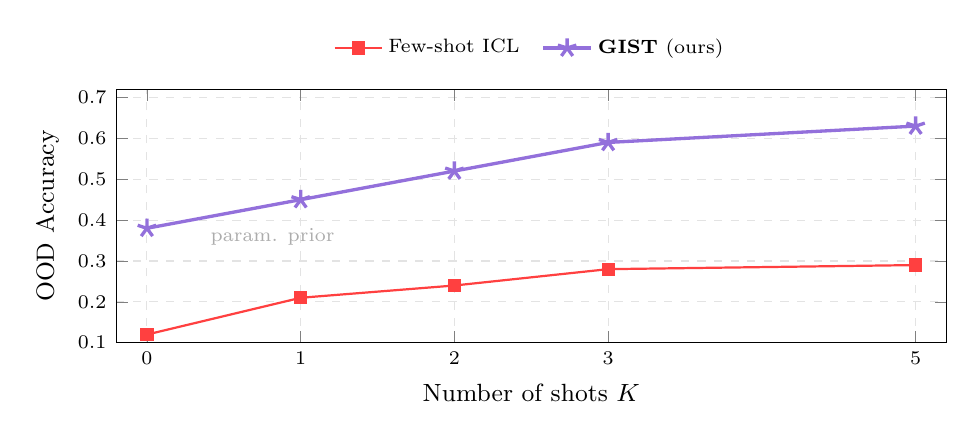
\begin{tikzpicture}
  \begin{axis}[
    xlabel       = {Number of shots $K$},
    ylabel       = {OOD Accuracy},
    xmin = -0.2, xmax = 5.2,
    ymin = 0.10, ymax = 0.72,
    xtick        = {0, 1, 2, 3, 5},
    ytick        = {0.1, 0.2, 0.3, 0.4, 0.5, 0.6, 0.7},
    yticklabel style = {font=\scriptsize},
    x tick label style = {font=\scriptsize},
    ylabel style = {font=\small},
    xlabel style = {font=\small},
    width        = \columnwidth,
    height       = 4.8cm,
    legend style = {at={(0.5,1.08)}, anchor=south,
                    font=\scriptsize, row sep=0pt,
                    legend columns=2,
                    draw=none, fill=none,
                    /tikz/every even column/.append style={column sep=6pt}},
    grid         = major,
    grid style   = {gray!22, dashed},
    clip         = false,
  ]
  \addplot[red!75, thick, mark=square*, mark size=2pt,
           mark options={fill=red!75}]
    coordinates {(0,0.12) (1,0.21) (2,0.24) (3,0.28) (5,0.29)};
  \addlegendentry{Few-shot ICL}
  \addplot[MediumPurple, very thick, mark=star, mark size=3.5pt,
           mark options={fill=MediumPurple}]
    coordinates {(0,0.38) (1,0.45) (2,0.52) (3,0.59) (5,0.63)};
  \addlegendentry{\textbf{\gist{}} (ours)}
  \node[gray!65, font=\tiny, align=center, anchor=west]
    at (axis cs:0.35, 0.36) {\scriptsize param. prior};
  \end{axis}
  \end{tikzpicture}
  \caption{OOD accuracy vs.\ shot count $K$.
    ICL saturates after $K{=}1$--$2$; \gist{} continues to improve as
    each additional example refines the \texttt{INDUCTIVE\_RULE} strategy.
    At $K{=}0$, \gist{} (0.38) outperforms $K{=}3$ ICL (0.28),
    confirming parametrically internalized inductive priors.}
  \label{fig:fewshot_util}
\end{figure}

\gist{} continues to benefit from additional demonstrations beyond $K{=}2$, unlike ICL which saturates early.
At $K{=}0$, \gist{} already outperforms $K{=}3$ ICL, confirming that meta-inductive priors are encoded as parametric knowledge independent of demonstration retrieval.

% ============================================================
\section{Additional Experiments}
\label{app:extra_results}

% ── Zero-shot and Habit-Zero-Shot Full Results ────────────────────────────────
\subsection{Zero-Shot and Habit-Zero-Shot Results}
\label{app:zero_shot_results}

Table~\ref{tab:zero_shot_results} completes the 2$\times$2 method matrix from Table~\ref{tab:main_results} by reporting zero-shot (\textbf{0S}) and habit-zero-shot (\textbf{H-0S}) results for all backbones.
\textbf{0S}: zero-shot direct answer (no demonstrations, no strategy step, $1\times$ cost).
\textbf{H-0S}: zero-shot strategy-then-answer via two calls to the same backbone ($2\times$ cost).
\textcolor{gray}{Gray}~$\Delta$\%: H-0S improvement over same-backbone 0S (OOD).
These rows are separated from the main table for space; all conclusions in the main text apply jointly to all four methods.

\begin{table*}[h]
  \centering
  \fontsize{6.8pt}{7.8pt}\selectfont
  \setlength{\tabcolsep}{2.2pt}
  \renewcommand{\arraystretch}{0.82}
  % Column map (8 columns): c1 Model  c2 Method
  %   c3 BBH  c4 ID (BIG-Bench)  c5 OOD+Δ%  c6 HM2  c7 Ling.  c8 Avg*
  \begin{tabular}{
    >{\raggedright\arraybackslash}p{1.4cm}%
    >{\raggedright\arraybackslash}p{1.7cm}%
    S[table-format=1.2]%
    S[table-format=1.2]%
    >{\centering\arraybackslash}p{1.35cm}%
    S[table-format=1.4]%
    S[table-format=1.4]%
    S[table-format=1.2]%
  }
    \toprule
    & & \multicolumn{1}{c}{} & \multicolumn{2}{c}{\textbf{BIG-Bench}} & & & \\[-5pt]
    \cmidrule(lr){4-5}
    \multicolumn{1}{c}{\textbf{Model}} &
    \multicolumn{1}{c}{\textbf{Method}} &
    \multicolumn{1}{c}{\textbf{BBH}} &
    \multicolumn{1}{c}{\textbf{ID}} &
    \multicolumn{1}{c}{\textbf{OOD} ($\Delta$\%)} &
    \multicolumn{1}{c}{\textbf{HM2}} &
    \multicolumn{1}{c}{\textbf{Ling.}} &
    \multicolumn{1}{c}{\textbf{Avg.}$^{*}$} \\
    \midrule
    %
    % ══════════════════════════════════════════════════════════
    \rowcolor{gray!8}
    \multicolumn{8}{l}{\textit{w/o RL Training}} \\[-2pt]
    \midrule
    % ══════════════════════════════════════════════════════════
    %
    \multirow{2}{*}{Gemma-3-4B}
      & \zs~0S   & {\cdash} & {\cdash} & {\cdash} & {\cdash} & {\cdash} & {\cdash} \\
      & \ho~H-0S & {\cdash} & {\cdash} & {\cdash} & {\cdash} & {\cdash} & {\cdash} \\
    \cmidrule(l){2-8}
    \multirow{2}{*}{Qwen3-4B}
      & \zs~0S   & {\cdash} & {\cdash} & {\cdash} & {\cdash} & {\cdash} & {\cdash} \\
      & \ho~H-0S & {\cdash} & {\cdash} & {\cdash} & {\cdash} & {\cdash} & {\cdash} \\
    \cmidrule(l){2-8}
    \multirow{2}{*}{Qwen3-8B}
      & \zs~0S   & {\cdash} & {\cdash} & {\cdash} & {\cdash} & {\cdash} & {\cdash} \\
      & \ho~H-0S & {\cdash} & {\cdash} & {\cdash} & {\cdash} & {\cdash} & {\cdash} \\
    \cmidrule(l){2-8}
    \multirow{2}{*}{Llama-3.1-8B}
      & \zs~0S   & {\cdash} & {\cdash} & {\cdash} & {\cdash} & {\cdash} & {\cdash} \\
      & \ho~H-0S & {\cdash} & {\cdash} & {\cdash} & {\cdash} & {\cdash} & {\cdash} \\
    \cmidrule(l){2-8}
    \multirow{2}{*}{Gemini$^{\dagger}$}
      & \zs~0S   & {\cdash} & {\cdash} & {\cdash} & {\cdash} & {\cdash} & {\cdash} \\
      & \ho~H-0S & {\cdash} & {\cdash} & {\cdash} & {\cdash} & {\cdash} & {\cdash} \\
    \cmidrule(l){2-8}
    \multirow{2}{*}{GPT-5$^{\dagger}$}
      & \zs~0S   & {\cdash} & {\cdash} & {\cdash} & {\cdash} & {\cdash} & {\cdash} \\
      & \ho~H-0S & {\cdash} & {\cdash} & {\cdash} & {\cdash} & {\cdash} & {\cdash} \\
    %
    % ══════════════════════════════════════════════════════════
    \midrule
    \rowcolor{gray!8}
    \multicolumn{8}{l}{\textit{w/ RL Training (Cross-task GRPO)}} \\[-2pt]
    \midrule
    % ══════════════════════════════════════════════════════════
    %
    % Col 1 (Model) uncolored so \multirow text is unobstructed.
    \multirow{2}{*}{Gemma-3-4B}
      & \cellcolor{rlbg}\zs~0S   & \cellcolor{rlbg}{\cdash} & \cellcolor{rlbg}{\cdash} & \cellcolor{rlbg}{\cdash} & \cellcolor{rlbg}{\cdash} & \cellcolor{rlbg}{\cdash} & \cellcolor{rlbg}{\cdash} \\
      & \cellcolor{rlbg}\ho~H-0S & \cellcolor{rlbg}{\cdash} & \cellcolor{rlbg}{\cdash} & \cellcolor{rlbg}{\cdash} & \cellcolor{rlbg}{\cdash} & \cellcolor{rlbg}{\cdash} & \cellcolor{rlbg}{\cdash} \\
    \cmidrule(l){2-8}
    \multirow{2}{*}{Qwen3-4B}
      & \cellcolor{rlbg}\zs~0S   & \cellcolor{rlbg}{\cdash} & \cellcolor{rlbg}{\cdash} & \cellcolor{rlbg}{\cdash} & \cellcolor{rlbg}{\cdash} & \cellcolor{rlbg}{\cdash} & \cellcolor{rlbg}{\cdash} \\
      & \cellcolor{rlbg}\ho~H-0S & \cellcolor{rlbg}{\cdash} & \cellcolor{rlbg}{\cdash} & \cellcolor{rlbg}{\cdash} & \cellcolor{rlbg}{\cdash} & \cellcolor{rlbg}{\cdash} & \cellcolor{rlbg}{\cdash} \\
    \cmidrule(l){2-8}
    \multirow{2}{*}{Qwen3-8B}
      & \cellcolor{rlbg}\zs~0S   & \cellcolor{rlbg}{\cdash} & \cellcolor{rlbg}{\cdash} & \cellcolor{rlbg}{\cdash} & \cellcolor{rlbg}{\cdash} & \cellcolor{rlbg}{\cdash} & \cellcolor{rlbg}{\cdash} \\
      & \cellcolor{rlbg}\ho~H-0S & \cellcolor{rlbg}{\cdash} & \cellcolor{rlbg}{\cdash} & \cellcolor{rlbg}{\cdash} & \cellcolor{rlbg}{\cdash} & \cellcolor{rlbg}{\cdash} & \cellcolor{rlbg}{\cdash} \\
    \cmidrule(l){2-8}
    \multirow{2}{*}{Llama-3.1-8B}
      & \cellcolor{rlbg}\zs~0S   & \cellcolor{rlbg}{\cdash} & \cellcolor{rlbg}{\cdash} & \cellcolor{rlbg}{\cdash} & \cellcolor{rlbg}{\cdash} & \cellcolor{rlbg}{\cdash} & \cellcolor{rlbg}{\cdash} \\
      & \cellcolor{rlbg}\ho~H-0S & \cellcolor{rlbg}{\cdash} & \cellcolor{rlbg}{\cdash} & \cellcolor{rlbg}{\cdash} & \cellcolor{rlbg}{\cdash} & \cellcolor{rlbg}{\cdash} & \cellcolor{rlbg}{\cdash} \\
    \bottomrule
  \end{tabular}
  \vspace{2pt}\\
  {\fontsize{5.8pt}{6.8pt}\selectfont
    $^{*}$~Avg.~$=$~mean of BBH, BIG-Bench ID, OOD (HM2 and Ling.\ excluded).
    \quad $^{\dagger}$~closed-source API, no fine-tuning.
    \quad \textcolor{gray}{Gray}~$\Delta$\%: H-0S over same-backbone 0S (OOD).
    \quad ``\cdash'': result pending.
  }
  \caption{Zero-shot (\textbf{0S}) and habit-zero-shot (\textbf{H-0S}) results, complementing Table~\ref{tab:main_results}.
    \textbf{0S}: zero-shot direct answer ($1\times$ inference cost).
    \textbf{H-0S}: zero-shot strategy-then-answer via two calls to the same backbone ($2\times$ cost).
    \textcolor{gray}{Gray}~$\Delta$\%: H-0S improvement over same-backbone 0S (OOD).
    \textbf{w/o~RL}: backbone off-the-shelf.
    \textbf{w/~RL}: backbone cross-task GRPO-trained (shaded rows).
    $\dagger$: closed-source API.
    ``\cdash'': result pending.}
  \label{tab:zero_shot_results}
\end{table*}

% ── Qwen3-8B Few-Shot Full Results ───────────────────────────────────────────
\subsection{Qwen3-8B Full Results}
\label{app:qwen38b}

Table~\ref{tab:qwen38b_results} reports full few-shot results for the Qwen3-8B backbone
(both w/o and w/ Training), separated from Table~\ref{tab:main_results} for space.
Column definitions and symbols follow Table~\ref{tab:main_results}.

\begin{table*}[h]
  \centering
  \fontsize{6.8pt}{7.8pt}\selectfont
  \setlength{\tabcolsep}{3pt}
  \renewcommand{\arraystretch}{0.82}
  \begin{tabular}{
    >{\centering\arraybackslash}p{0.75cm}%   c1 Type (rotated label)
    >{\raggedright\arraybackslash}p{1.5cm}%  c2 Model
    @{\hskip 12pt}%                          extra gap: Model → Method
    >{\raggedright\arraybackslash}p{1.2cm}%  c3 Method
    S[table-format=2.1]%                     c4 BBH
    S[table-format=2.1]%                     c5 BIG-Bench ID
    >{\centering\arraybackslash}p{1.35cm}%   c6 BIG-Bench OOD+Δ%
    S[table-format=2.1]%                     c7 Avg*
    S[table-format=1.1]%                     c8 HM2
    S[table-format=2.1]%                     c9 Ling.
  }
    \toprule
    & & & & \multicolumn{2}{c}{\textbf{BIG-Bench}} & & & \\[-2pt]
    \cmidrule(lr){5-6}
    \multicolumn{1}{c}{\textbf{Type}} &
    \multicolumn{1}{c}{\textbf{Model}} &
    \multicolumn{1}{c}{\textbf{Method}} &
    \multicolumn{1}{c}{\textbf{BBH}} &
    \multicolumn{1}{c}{\textbf{ID} ($\Delta$\%)} &
    \multicolumn{1}{c}{\textbf{OOD} ($\Delta$\%)} &
    \multicolumn{1}{c}{\textbf{Avg.}$^{*}$} &
    \multicolumn{1}{c}{\textbf{HM2}} &
    \multicolumn{1}{c}{\textbf{Ling.}} \\
    \midrule
    % ── w/o Training ──────────────────────────── 2 rows ──
    \multirow{2}{*}{\rotatebox{90}{\textit{w/o Training}}}
      & \multirow{2}{*}{Qwen3-8B}
        & \fs~FS   & 31.48 & 21.33 & 28.33 & 27.0 & 0.47 & 0.0 \\
    & & \hf~H-FS & 38.15 & 39.00 & 52.67 & 43.0 & 1.42 & 0.0 \\
    \midrule
    % ── w/ Training ───────────────────────────── 2 rows ──
    \multirow{2}{*}{\rotatebox{90}{\textit{w/ Training}}}
      & \multirow{2}{*}{Qwen3-8B}
        & \cellcolor{rlbg}\fs~FS   & \cellcolor{rlbg}47.0 & \cellcolor{rlbg}41.0 & \cellcolor{rlbg}65.0 & \cellcolor{rlbg}51.0 & \cellcolor{rlbg}0.3 & \cellcolor{rlbg}0.0 \\
    & & \cellcolor{mist}\hf~\textbf{\gist{}} & \multicolumn{1}{c}{\cellcolor{mist}\textbf{48.0}\,\dr{55}} & \multicolumn{1}{c}{\cellcolor{mist}\textbf{62.0}\,\dr{195}} & \cellcolor{mist}\textbf{49.0}\,\dr{75} & \cellcolor{mist}53.0 & \cellcolor{mist}2.4 & \cellcolor{mist}0.0 \\
    \bottomrule
  \end{tabular}
  \vspace{2pt}\\
  {\fontsize{5.8pt}{6.8pt}\selectfont
    $^{*}$~Avg.~$=$~(BBH $+$ BIG-Bench ID $+$ OOD) $/$ 3.
    \quad \textcolor{BrickRed}{Red}~$\Delta$\%: \gist{} improvement over same-backbone FS (OOD).
    \quad ``\cdash'': result pending.
  }
  \caption{Qwen3-8B results (few-shot \textbf{FS} and \textbf{\gist{}}), complementing
    Table~\ref{tab:main_results}.
    \textbf{w/o~Training}: backbone used off-the-shelf.
    \textbf{w/~Training}: backbone cross-task GRPO-trained (shaded rows).
    Column definitions and symbols follow Table~\ref{tab:main_results}.}
  \label{tab:qwen38b_results}
\end{table*}

\subsection{Full Zero-Shot SG Scale Sweep}
\label{app:scale_sweep}

\begin{table}[H]
  \centering
  \small
  \setlength{\tabcolsep}{4pt}
  \renewcommand{\arraystretch}{1.12}
  \resizebox{\columnwidth}{!}{%
  \begin{tabular}{lcccc}
    \toprule
    \textbf{SG (No RL)} & \textbf{ID}${\uparrow}$ & \textbf{BBH}${\uparrow}$ & \textbf{OOD}${\uparrow}$ & \textbf{OOD RI\%} \\
    \midrule
    Qwen3-1.7B + AS-4B & \cdash & \cdash & \cdash & \cdash \\
    Qwen3-4B   + AS-4B & 0.28   & \cdash & \cdash & \cdash \\
    Qwen3-8B   + AS-4B & \cdash & \cdash & \cdash & \cdash \\
    Qwen3-14B  + AS-4B & \cdash & \cdash & \cdash & \cdash \\
    Qwen3-32B  + AS-4B & \cdash & \cdash & \cdash & \cdash \\
    \midrule
    \rowcolor{MediumPurple!10}
    \textbf{\gist{}} (SG-4B + AS-4B) & \textbf{0.46} & \textbf{0.78} & \textbf{0.59} & \textbf{+149\%} \\
    \bottomrule
  \end{tabular}%
  }
  \caption{Full zero-shot SG scale sweep (1.7B--32B) with AS fixed at Qwen3-4B, compared to \gist{}-4B. \gist{}-4B surpasses all zero-shot variants including SG-32B, confirming that meta-inductive habits are orthogonal to parameter count.}
  \label{tab:scale_sweep}
\end{table}

\subsection{Sensitivity to Shot Count \texorpdfstring{$K$}{K}}
\label{app:k_sensitivity}

\begin{table}[H]
  \centering
  \small
  \setlength{\tabcolsep}{6pt}
  \renewcommand{\arraystretch}{1.15}
  \begin{tabular}{cccc}
    \toprule
    $K$ & \textbf{ID} $\text{Acc}{\uparrow}$ & \textbf{BBH} ${\uparrow}$ & \textbf{OOD} ${\uparrow}$ \\
    \midrule
    0           & \cdash          & \cdash          & \cdash   \\
    1           & \cdash          & \cdash          & \cdash   \\
    2           & \cdash          & \cdash          & \cdash   \\
    3$^\dagger$ & \textbf{0.46}   & \textbf{0.78}   & \textbf{0.59}   \\
    5           & \cdash          & \cdash          & \cdash   \\
    \bottomrule
  \end{tabular}
  \caption{Sensitivity to shot count $K$ ($^\dagger$: default). Significant accuracy at $K{=}0$ confirms that meta-inductive priors are internalized as parametric knowledge.}
  \label{tab:k_sensitivity}
\end{table}

At $K{=}0$ (zero-shot, task description only), effective strategy generation by \sg{} would confirm that meta-inductive priors have been internalized as parametric knowledge---the strongest evidence for learn-to-induce. Insufficient examples ($K{=}1$) limit induction quality; excessive examples risk over-specializing the strategy to the current task. $K{=}3$ is the default optimal trade-off (full data pending).

\subsection{Sensitivity to ICR Log-Smoothing Constant \texorpdfstring{$k$}{k}}
\label{app:icr_k}

ICR 中的对数平滑常数 $k$（式~\eqref{eq:eir}）控制奖励对增益幅度的压缩程度：$k$ 越大，较大增益所获奖励的相对优势越显著；$k$ 越小，奖励分布越平坦。我们以默认配置（EIR+ICR，$M{=}4$，$K{=}3$）固定其余超参数，在 $k \in \{1, 5, 10, 20\}$ 上扫描。

\begin{table}[H]
  \centering
  \small
  \setlength{\tabcolsep}{6pt}
  \renewcommand{\arraystretch}{1.15}
  \begin{tabular}{cccc}
    \toprule
    $k$ & \textbf{ID} ${\uparrow}$ & \textbf{BBH} ${\uparrow}$ & \textbf{OOD} ${\uparrow}$ \\
    \midrule
    1           & \cdash & \cdash & \cdash \\
    5           & \cdash & \cdash & \cdash \\
    10$^\dagger$ & \textbf{0.65} & \textbf{0.78} & \textbf{0.60} \\
    20          & \cdash & \cdash & \cdash \\
    \bottomrule
  \end{tabular}
  \caption{Sensitivity to ICR log-smoothing constant $k$ ($^\dagger$: default $k{=}10$).
    Performance is relatively stable across $k \in [5, 10]$;
    very small $k$ ($=1$) flattens reward distinctions while very large $k$ ($=20$) amplifies noise on near-zero gains. ``\cdash'': pending.}
  \label{tab:icr_k}
\end{table}

$k{=}10$ 在稳定性与区分度之间取得最优平衡，且结果对 $k$ 并不敏感（$k \in [5, 10]$ 区间性能相近），表明 EIR 的核心设计（难度归一化与符号传递）是主要贡献，$k$ 的精确取值为次要因素。

%% TODO: Add the following
%% 1. Reward training curves (R_fmt fast convergence; R_exec gradual improvement)
%% 2. Per-subtask breakdown for BBH (27 subtasks)

\end{document}
